\documentclass[10pt]{beamer}
\usepackage[utf8]{inputenc}
\usepackage{tikz, pgfplots}
\pgfplotsset{compat=1.18}
\usetikzlibrary{positioning}
\usetikzlibrary{trees}
\usetikzlibrary{shapes.geometric, arrows.meta, positioning}
\usepackage{xcolor}
\usepackage{graphicx}
\usepackage{subcaption}
\usepackage{hyperref} 
\usepackage{colortbl} % Required for \rowcolor
\usepackage{animate}
\usepackage[T1]{fontenc}
\usepackage{amsmath, amsfonts, amssymb}
\usepackage[french]{babel}
\usepackage[normalem]{ulem}

% Theme và màu sắc cho beamer
\usetheme{AnnArbor}
\usecolortheme{seahorse}

% Định nghĩa và thiết lập màu sắc chung
\definecolor{mydarkblue}{RGB}{0,51,102}
\setbeamercolor{structure}{fg=mydarkblue}
\setbeamercolor{frametitle}{bg=mydarkblue, fg=white}
\setbeamercolor{title}{fg=mydarkblue}
\setbeamercolor{item}{fg=mydarkblue}
\setbeamercolor{block title}{bg=mydarkblue, fg=white}
\setbeamercolor{block body}{bg=white, fg=black}
\setbeamercolor{section in toc}{fg=mydarkblue}
\setbeamercolor{subsection in toc}{fg=mydarkblue}
\setbeamercolor{caption name}{fg=mydarkblue}
\setbeamercolor{author}{fg=mydarkblue}
\setbeamercolor{date}{fg=mydarkblue}
\setbeamercolor{institute}{fg=mydarkblue}
\setbeamertemplate{caption}[numbered]
\usepackage{multirow}
\title{Rapport Hebdo}
\author{Viet Anh Quach}
\institute{3SR}
\date{\today}

\begin{document}

\begin{frame}
    \titlepage
\end{frame}


\section{DEM}
% \begin{frame}{Changer le modèle}
%     \begin{figure}[h]
%         \centering
%         \scalebox{0.15}{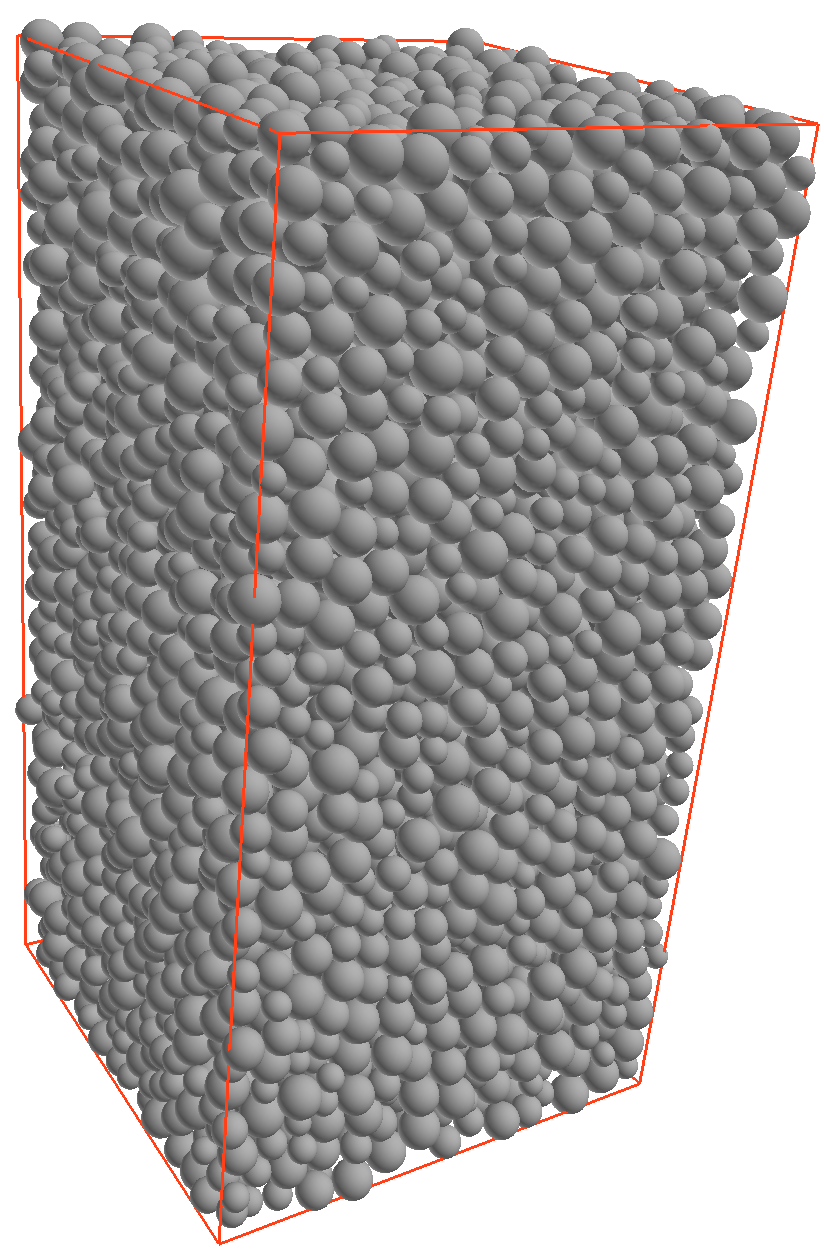
\includegraphics{rentangulaire.png}}
%         \caption{Boîte rentangulaire}
%     \end{figure}
% \end{frame}


% \begin{frame}{Étude sur le nombre d'inertie}
%     \begin{table}
%         \centering
%         \begin{tabular}{|c|c|c|c|}
%             \hline
%             \textbf{Symboles}               & \textbf{Paramètres} & \textbf{Valeurs}                      & \textbf{Unité}  \\
%             \hline
%             Nombre de particules            & N                   & $15 \times 30 \times 15 = 6750$       & -               \\
%             \hline
%             Le rayon des particules         & R                   & 0.003 $\div$ 0.005                    & m               \\
%             \hline
%             Masse volumique                 & $\rho$              & 2500                                  & $\text{kg/m}^3$ \\
%             \hline
%             Raideur normale et tangentielle & $k_n$ \& $k_t$      & \textcolor{black}{$3 \times 10^6$}    & $\text{N/m}$    \\
%             \hline
%             Niveau de raideur               & $\kappa$            & >1000                                 & -               \\
%             \hline
%             Coefficient de frottement       & $\mu$               & $\mu_{iso} = 0.1, \mu_{triax} = 0.5 $ & -               \\
%             \hline
%             Coefficient d'amortissement     & $\alpha$            & 0.0                                   & -               \\
%             \hline
%         \end{tabular}
%         \caption{Valeurs gardé}
%     \end{table}
% \end{frame}


% \begin{frame}{Étude sur le nombre d'inertie}
%     \begin{columns}
%         \begin{column}{0.5\textwidth}
%             \begin{table}
%                 \centering
%                 \begin{tabular}{|c|c|c|c|}
%                     \hline
%                     % \textbf{v (m/s) \&P (kPa)} & $3 \times 10^4$ & $3 \times 10^2$                       & $3 \times 10^0$ & $3 \times 10^{-2}$ & $3 \times 10^{-4}$ \\
%                     $v $(m/s)                & $ \sigma_3 = 3 \times 10^2$ (kPa) \\
%                     \hline
%                     $4.542   \times 10^{-3}$ & I = $10^{-5}$                     \\
%                     \hline
%                     $4.542   \times 10^{-2}$ & I = $10^{-4}$                     \\
%                     \hline
%                     $4.542   \times 10^{-1}$ & I = $10^{-3}$                     \\
%                     \hline
%                     $4.542   \times 10^{0}$  & I = $10^{-2}$                     \\
%                     \hline
%                     $4.542   \times 10^{1}$  & I = $10^{-1}$                     \\
%                     \hline
%                     $4.542   \times 10^{2}$  & I = $1$                           \\
%                     \hline
%                 \end{tabular}
%                 \caption{Changer la vitesse}
%             \end{table}
%         \end{column}
%         \begin{column}{0.5\textwidth}
%             \begin{table}
%                 \centering
%                 \begin{tabular}{|c|c|c|c|}
%                     \hline
%                     % \textbf{v (m/s) \&P (kPa)} & $3 \times 10^4$ & $3 \times 10^2$                       & $3 \times 10^0$ & $3 \times 10^{-2}$ & $3 \times 10^{-4}$ \\
%                     $\sigma_{3} $(kPa) & v $ = 4.542   \times 10^{-2}$ (m/s) \\
%                     \hline
%                     $3 \times 10^4$    & I = $10^{-5}$                       \\
%                     \hline
%                     $3 \times 10^2$    & I = $10^{-4}$                       \\
%                     \hline
%                     $3 \times 10^0$    & I = $10^{-3}$                       \\
%                     \hline
%                     $3 \times 10^{-2}$ & I = $10^{-2}$                       \\
%                     \hline
%                     $3 \times 10^{-4}$ & I = $10^{-1}$                       \\
%                     \hline
%                     $3 \times 10^{-7}$ & I = $1$                             \\
%                     \hline
%                 \end{tabular}
%                 \caption{Changer la contrainte de confinement}
%             \end{table}
%         \end{column}
%     \end{columns}
% \end{frame}

% \begin{frame}{Changer la contrainte}
%     \begin{columns}
%         \begin{column}{0.5\textwidth}
%             \begin{figure}[h]
%                 \centering
%                 \scalebox{0.5}{% GNUPLOT: LaTeX picture with Postscript
\begingroup
  \makeatletter
  \providecommand\color[2][]{%
    \GenericError{(gnuplot) \space\space\space\@spaces}{%
      Package color not loaded in conjunction with
      terminal option `colourtext'%
    }{See the gnuplot documentation for explanation.%
    }{Either use 'blacktext' in gnuplot or load the package
      color.sty in LaTeX.}%
    \renewcommand\color[2][]{}%
  }%
  \providecommand\includegraphics[2][]{%
    \GenericError{(gnuplot) \space\space\space\@spaces}{%
      Package graphicx or graphics not loaded%
    }{See the gnuplot documentation for explanation.%
    }{The gnuplot epslatex terminal needs graphicx.sty or graphics.sty.}%
    \renewcommand\includegraphics[2][]{}%
  }%
  \providecommand\rotatebox[2]{#2}%
  \@ifundefined{ifGPcolor}{%
    \newif\ifGPcolor
    \GPcolortrue
  }{}%
  \@ifundefined{ifGPblacktext}{%
    \newif\ifGPblacktext
    \GPblacktextfalse
  }{}%
  % define a \g@addto@macro without @ in the name:
  \let\gplgaddtomacro\g@addto@macro
  % define empty templates for all commands taking text:
  \gdef\gplbacktext{}%
  \gdef\gplfronttext{}%
  \makeatother
  \ifGPblacktext
    % no textcolor at all
    \def\colorrgb#1{}%
    \def\colorgray#1{}%
  \else
    % gray or color?
    \ifGPcolor
      \def\colorrgb#1{\color[rgb]{#1}}%
      \def\colorgray#1{\color[gray]{#1}}%
      \expandafter\def\csname LTw\endcsname{\color{white}}%
      \expandafter\def\csname LTb\endcsname{\color{black}}%
      \expandafter\def\csname LTa\endcsname{\color{black}}%
      \expandafter\def\csname LT0\endcsname{\color[rgb]{1,0,0}}%
      \expandafter\def\csname LT1\endcsname{\color[rgb]{0,1,0}}%
      \expandafter\def\csname LT2\endcsname{\color[rgb]{0,0,1}}%
      \expandafter\def\csname LT3\endcsname{\color[rgb]{1,0,1}}%
      \expandafter\def\csname LT4\endcsname{\color[rgb]{0,1,1}}%
      \expandafter\def\csname LT5\endcsname{\color[rgb]{1,1,0}}%
      \expandafter\def\csname LT6\endcsname{\color[rgb]{0,0,0}}%
      \expandafter\def\csname LT7\endcsname{\color[rgb]{1,0.3,0}}%
      \expandafter\def\csname LT8\endcsname{\color[rgb]{0.5,0.5,0.5}}%
    \else
      % gray
      \def\colorrgb#1{\color{black}}%
      \def\colorgray#1{\color[gray]{#1}}%
      \expandafter\def\csname LTw\endcsname{\color{white}}%
      \expandafter\def\csname LTb\endcsname{\color{black}}%
      \expandafter\def\csname LTa\endcsname{\color{black}}%
      \expandafter\def\csname LT0\endcsname{\color{black}}%
      \expandafter\def\csname LT1\endcsname{\color{black}}%
      \expandafter\def\csname LT2\endcsname{\color{black}}%
      \expandafter\def\csname LT3\endcsname{\color{black}}%
      \expandafter\def\csname LT4\endcsname{\color{black}}%
      \expandafter\def\csname LT5\endcsname{\color{black}}%
      \expandafter\def\csname LT6\endcsname{\color{black}}%
      \expandafter\def\csname LT7\endcsname{\color{black}}%
      \expandafter\def\csname LT8\endcsname{\color{black}}%
    \fi
  \fi
    \setlength{\unitlength}{0.0500bp}%
    \ifx\gptboxheight\undefined%
      \newlength{\gptboxheight}%
      \newlength{\gptboxwidth}%
      \newsavebox{\gptboxtext}%
    \fi%
    \setlength{\fboxrule}{0.5pt}%
    \setlength{\fboxsep}{1pt}%
    \definecolor{tbcol}{rgb}{1,1,1}%
\begin{picture}(7200.00,5040.00)%
    \gplgaddtomacro\gplbacktext{%
      \csname LTb\endcsname%%
      \put(1210,1144){\makebox(0,0)[r]{\strut{}$0$}}%
      \csname LTb\endcsname%%
      \put(1210,1512){\makebox(0,0)[r]{\strut{}$0.0002$}}%
      \csname LTb\endcsname%%
      \put(1210,1879){\makebox(0,0)[r]{\strut{}$0.0004$}}%
      \csname LTb\endcsname%%
      \put(1210,2247){\makebox(0,0)[r]{\strut{}$0.0006$}}%
      \csname LTb\endcsname%%
      \put(1210,2614){\makebox(0,0)[r]{\strut{}$0.0008$}}%
      \csname LTb\endcsname%%
      \put(1210,2982){\makebox(0,0)[r]{\strut{}$0.001$}}%
      \csname LTb\endcsname%%
      \put(1210,3349){\makebox(0,0)[r]{\strut{}$0.0012$}}%
      \csname LTb\endcsname%%
      \put(1210,3717){\makebox(0,0)[r]{\strut{}$0.0014$}}%
      \csname LTb\endcsname%%
      \put(1210,4084){\makebox(0,0)[r]{\strut{}$0.0016$}}%
      \csname LTb\endcsname%%
      \put(1210,4452){\makebox(0,0)[r]{\strut{}$0.0018$}}%
      \csname LTb\endcsname%%
      \put(1210,4819){\makebox(0,0)[r]{\strut{}$0.002$}}%
      \csname LTb\endcsname%%
      \put(1342,924){\makebox(0,0){\strut{}$0$}}%
      \csname LTb\endcsname%%
      \put(1978,924){\makebox(0,0){\strut{}$10$}}%
      \csname LTb\endcsname%%
      \put(2613,924){\makebox(0,0){\strut{}$20$}}%
      \csname LTb\endcsname%%
      \put(3249,924){\makebox(0,0){\strut{}$30$}}%
      \csname LTb\endcsname%%
      \put(3884,924){\makebox(0,0){\strut{}$40$}}%
      \csname LTb\endcsname%%
      \put(4520,924){\makebox(0,0){\strut{}$50$}}%
      \csname LTb\endcsname%%
      \put(5155,924){\makebox(0,0){\strut{}$60$}}%
      \csname LTb\endcsname%%
      \put(5791,924){\makebox(0,0){\strut{}$70$}}%
      \put(5923,1144){\makebox(0,0)[l]{\strut{}$-0.5$}}%
      \put(5923,1512){\makebox(0,0)[l]{\strut{}$0$}}%
      \put(5923,1879){\makebox(0,0)[l]{\strut{}$0.5$}}%
      \put(5923,2247){\makebox(0,0)[l]{\strut{}$1$}}%
      \put(5923,2614){\makebox(0,0)[l]{\strut{}$1.5$}}%
      \put(5923,2982){\makebox(0,0)[l]{\strut{}$2$}}%
      \put(5923,3349){\makebox(0,0)[l]{\strut{}$2.5$}}%
      \put(5923,3717){\makebox(0,0)[l]{\strut{}$3$}}%
      \put(5923,4084){\makebox(0,0)[l]{\strut{}$3.5$}}%
      \put(5923,4452){\makebox(0,0)[l]{\strut{}$4$}}%
      \put(5923,4819){\makebox(0,0)[l]{\strut{}$4.5$}}%
    }%
    \gplgaddtomacro\gplfronttext{%
      \csname LTb\endcsname%%
      \put(341,2981){\rotatebox{-270}{\makebox(0,0){\strut{}q (kPa)}}}%
      \put(6693,2981){\rotatebox{-270}{\makebox(0,0){\strut{}$\varepsilon_v$ (\%)}}}%
      \put(3566,594){\makebox(0,0){\strut{}$\varepsilon_{yy}$ (\%)}}%
      \csname LTb\endcsname%%
      \put(2711,393){\makebox(0,0)[r]{\strut{}$\sigma_3 = 3 \times 10^{-2}$ kPa}}%
      \csname LTb\endcsname%%
      \put(2711,173){\makebox(0,0)[r]{\strut{}$\sigma_3 = 3 \times 10^{0}$ kPa}}%
      \csname LTb\endcsname%%
      \put(5810,393){\makebox(0,0)[r]{\strut{}$\sigma_3 = 3 \times 10^{2}$ kPa}}%
    }%
    \gplbacktext
    \put(0,0){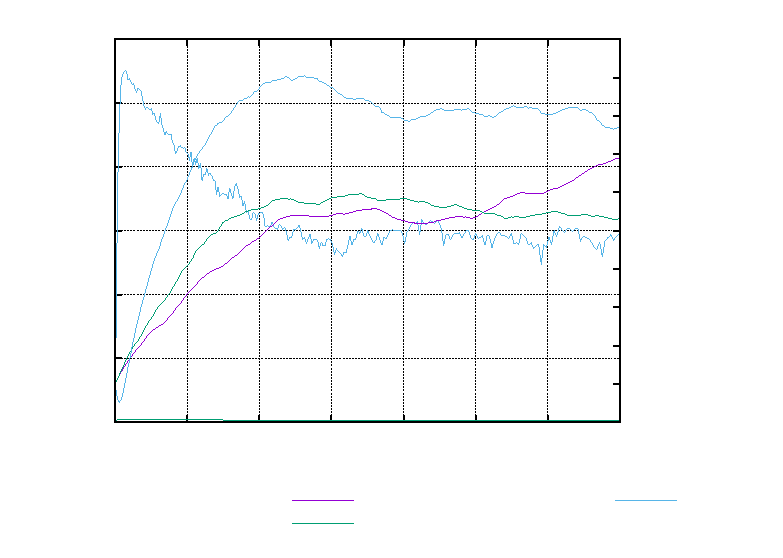
\includegraphics[width={360.00bp},height={252.00bp}]{./Contrainte_contrainteDeviatorique}}%
    \gplfronttext
  \end{picture}%
\endgroup
}
%                 \caption{Contrainte - Déformation DEM (changer la vitesse)}
%             \end{figure}
%         \end{column}
%         \begin{column}{0.5\textwidth}
%             \begin{table}
%                 \centering
%                 \begin{tabular}{|c|c|c|c|}
%                     \hline
%                     % \textbf{v (m/s) \&P (kPa)} & $3 \times 10^4$ & $3 \times 10^2$                       & $3 \times 10^0$ & $3 \times 10^{-2}$ & $3 \times 10^{-4}$ \\
%                     $\sigma_{3} $(kPa)      & v $ = 4.542   \times 10^{-2}$ (m/s)                  \\
%                     \hline
%                     $3 \times 10^4$         & $\kappa > 1000$                                      \\
%                     \hline
%                     $3 \times 10^2$         & I = $10^{-4}$                                        \\
%                     \hline
%                     \rowcolor{white}
%                     $3 \times 10^0$         & \multirow{2}{*}{$\tan {\varphi} \approx 90 \degres$} \\
%                     \cline{1-1}
%                     $3 \times 10^{-2}$      &                                                      \\
%                     \hline

%                     $4.542   \times 10^{1}$ & \multirow{2}{*}{IsoComp stabilise pas}               \\
%                     \cline{1-1}
%                     $4.542   \times 10^{2}$ &                                                      \\
%                     \hline
%                 \end{tabular}
%                 \caption{Changer la contrainte de confinement}
%             \end{table}
%         \end{column}
%     \end{columns}
% \end{frame}

% \begin{frame}{Changer la vitesse}
%     \begin{columns}
%         \begin{column}{0.5\textwidth}
%             \begin{figure}[h]
%                 \centering
%                 \scalebox{0.5}{% GNUPLOT: LaTeX picture with Postscript
\begingroup
  \makeatletter
  \providecommand\color[2][]{%
    \GenericError{(gnuplot) \space\space\space\@spaces}{%
      Package color not loaded in conjunction with
      terminal option `colourtext'%
    }{See the gnuplot documentation for explanation.%
    }{Either use 'blacktext' in gnuplot or load the package
      color.sty in LaTeX.}%
    \renewcommand\color[2][]{}%
  }%
  \providecommand\includegraphics[2][]{%
    \GenericError{(gnuplot) \space\space\space\@spaces}{%
      Package graphicx or graphics not loaded%
    }{See the gnuplot documentation for explanation.%
    }{The gnuplot epslatex terminal needs graphicx.sty or graphics.sty.}%
    \renewcommand\includegraphics[2][]{}%
  }%
  \providecommand\rotatebox[2]{#2}%
  \@ifundefined{ifGPcolor}{%
    \newif\ifGPcolor
    \GPcolortrue
  }{}%
  \@ifundefined{ifGPblacktext}{%
    \newif\ifGPblacktext
    \GPblacktextfalse
  }{}%
  % define a \g@addto@macro without @ in the name:
  \let\gplgaddtomacro\g@addto@macro
  % define empty templates for all commands taking text:
  \gdef\gplbacktext{}%
  \gdef\gplfronttext{}%
  \makeatother
  \ifGPblacktext
    % no textcolor at all
    \def\colorrgb#1{}%
    \def\colorgray#1{}%
  \else
    % gray or color?
    \ifGPcolor
      \def\colorrgb#1{\color[rgb]{#1}}%
      \def\colorgray#1{\color[gray]{#1}}%
      \expandafter\def\csname LTw\endcsname{\color{white}}%
      \expandafter\def\csname LTb\endcsname{\color{black}}%
      \expandafter\def\csname LTa\endcsname{\color{black}}%
      \expandafter\def\csname LT0\endcsname{\color[rgb]{1,0,0}}%
      \expandafter\def\csname LT1\endcsname{\color[rgb]{0,1,0}}%
      \expandafter\def\csname LT2\endcsname{\color[rgb]{0,0,1}}%
      \expandafter\def\csname LT3\endcsname{\color[rgb]{1,0,1}}%
      \expandafter\def\csname LT4\endcsname{\color[rgb]{0,1,1}}%
      \expandafter\def\csname LT5\endcsname{\color[rgb]{1,1,0}}%
      \expandafter\def\csname LT6\endcsname{\color[rgb]{0,0,0}}%
      \expandafter\def\csname LT7\endcsname{\color[rgb]{1,0.3,0}}%
      \expandafter\def\csname LT8\endcsname{\color[rgb]{0.5,0.5,0.5}}%
    \else
      % gray
      \def\colorrgb#1{\color{black}}%
      \def\colorgray#1{\color[gray]{#1}}%
      \expandafter\def\csname LTw\endcsname{\color{white}}%
      \expandafter\def\csname LTb\endcsname{\color{black}}%
      \expandafter\def\csname LTa\endcsname{\color{black}}%
      \expandafter\def\csname LT0\endcsname{\color{black}}%
      \expandafter\def\csname LT1\endcsname{\color{black}}%
      \expandafter\def\csname LT2\endcsname{\color{black}}%
      \expandafter\def\csname LT3\endcsname{\color{black}}%
      \expandafter\def\csname LT4\endcsname{\color{black}}%
      \expandafter\def\csname LT5\endcsname{\color{black}}%
      \expandafter\def\csname LT6\endcsname{\color{black}}%
      \expandafter\def\csname LT7\endcsname{\color{black}}%
      \expandafter\def\csname LT8\endcsname{\color{black}}%
    \fi
  \fi
    \setlength{\unitlength}{0.0500bp}%
    \ifx\gptboxheight\undefined%
      \newlength{\gptboxheight}%
      \newlength{\gptboxwidth}%
      \newsavebox{\gptboxtext}%
    \fi%
    \setlength{\fboxrule}{0.5pt}%
    \setlength{\fboxsep}{1pt}%
    \definecolor{tbcol}{rgb}{1,1,1}%
\begin{picture}(7200.00,5040.00)%
    \gplgaddtomacro\gplbacktext{%
      \csname LTb\endcsname%%
      \put(1210,1144){\makebox(0,0)[r]{\strut{}$-10000$}}%
      \csname LTb\endcsname%%
      \put(1210,1478){\makebox(0,0)[r]{\strut{}$-8000$}}%
      \csname LTb\endcsname%%
      \put(1210,1812){\makebox(0,0)[r]{\strut{}$-6000$}}%
      \csname LTb\endcsname%%
      \put(1210,2146){\makebox(0,0)[r]{\strut{}$-4000$}}%
      \csname LTb\endcsname%%
      \put(1210,2480){\makebox(0,0)[r]{\strut{}$-2000$}}%
      \csname LTb\endcsname%%
      \put(1210,2814){\makebox(0,0)[r]{\strut{}$0$}}%
      \csname LTb\endcsname%%
      \put(1210,3149){\makebox(0,0)[r]{\strut{}$2000$}}%
      \csname LTb\endcsname%%
      \put(1210,3483){\makebox(0,0)[r]{\strut{}$4000$}}%
      \csname LTb\endcsname%%
      \put(1210,3817){\makebox(0,0)[r]{\strut{}$6000$}}%
      \csname LTb\endcsname%%
      \put(1210,4151){\makebox(0,0)[r]{\strut{}$8000$}}%
      \csname LTb\endcsname%%
      \put(1210,4485){\makebox(0,0)[r]{\strut{}$10000$}}%
      \csname LTb\endcsname%%
      \put(1210,4819){\makebox(0,0)[r]{\strut{}$12000$}}%
      \csname LTb\endcsname%%
      \put(1342,924){\makebox(0,0){\strut{}$0$}}%
      \csname LTb\endcsname%%
      \put(1996,924){\makebox(0,0){\strut{}$10$}}%
      \csname LTb\endcsname%%
      \put(2651,924){\makebox(0,0){\strut{}$20$}}%
      \csname LTb\endcsname%%
      \put(3305,924){\makebox(0,0){\strut{}$30$}}%
      \csname LTb\endcsname%%
      \put(3960,924){\makebox(0,0){\strut{}$40$}}%
      \csname LTb\endcsname%%
      \put(4614,924){\makebox(0,0){\strut{}$50$}}%
      \csname LTb\endcsname%%
      \put(5269,924){\makebox(0,0){\strut{}$60$}}%
      \csname LTb\endcsname%%
      \put(5923,924){\makebox(0,0){\strut{}$70$}}%
      \put(6055,1144){\makebox(0,0)[l]{\strut{}$-50$}}%
      \put(6055,1757){\makebox(0,0)[l]{\strut{}$0$}}%
      \put(6055,2369){\makebox(0,0)[l]{\strut{}$50$}}%
      \put(6055,2982){\makebox(0,0)[l]{\strut{}$100$}}%
      \put(6055,3594){\makebox(0,0)[l]{\strut{}$150$}}%
      \put(6055,4207){\makebox(0,0)[l]{\strut{}$200$}}%
      \put(6055,4819){\makebox(0,0)[l]{\strut{}$250$}}%
    }%
    \gplgaddtomacro\gplfronttext{%
      \csname LTb\endcsname%%
      \put(341,2981){\rotatebox{-270}{\makebox(0,0){\strut{}q (kPa)}}}%
      \put(6693,2981){\rotatebox{-270}{\makebox(0,0){\strut{}$\varepsilon_v$ (\%)}}}%
      \put(3632,594){\makebox(0,0){\strut{}$\varepsilon_{yy}$ (\%)}}%
      \csname LTb\endcsname%%
      \put(1822,393){\makebox(0,0)[r]{\strut{}I $= 10^{-5}$}}%
      \csname LTb\endcsname%%
      \put(1822,173){\makebox(0,0)[r]{\strut{}I $= 10^{-4}$}}%
      \csname LTb\endcsname%%
      \put(3733,393){\makebox(0,0)[r]{\strut{}I $= 10^{-3}$}}%
      \csname LTb\endcsname%%
      \put(3733,173){\makebox(0,0)[r]{\strut{}I $= 10^{-2}$}}%
      \csname LTb\endcsname%%
      \put(5644,393){\makebox(0,0)[r]{\strut{}I $= 10^{-1}$}}%
      \csname LTb\endcsname%%
      \put(5644,173){\makebox(0,0)[r]{\strut{}I $= 10^{-0}$}}%
    }%
    \gplbacktext
    \put(0,0){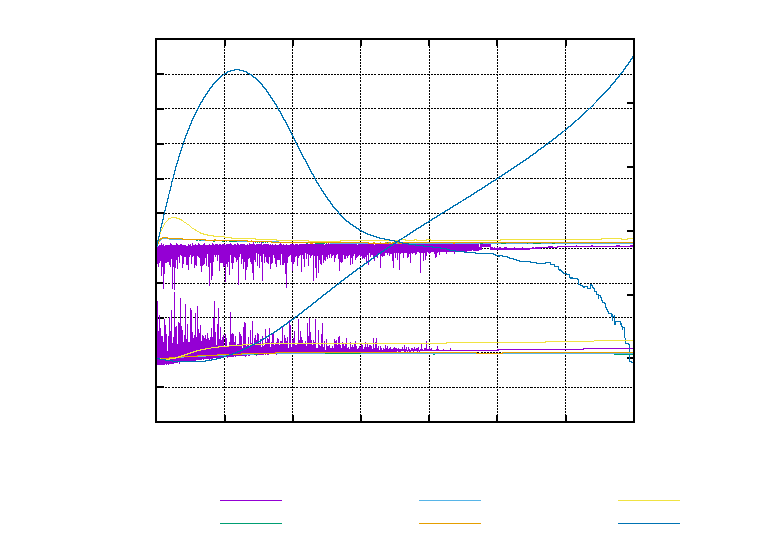
\includegraphics[width={360.00bp},height={252.00bp}]{./Vitess-contrainteDeviatorique}}%
    \gplfronttext
  \end{picture}%
\endgroup
}
%                 \caption{Contrainte - Déformation DEM (changer la vitesse)}
%             \end{figure}
%         \end{column}
%         \begin{column}{0.5\textwidth}
%             \begin{table}
%                 \centering
%                 \begin{tabular}{|c|c|c|c|}
%                     \hline
%                     % \textbf{v (m/s) \&P (kPa)} & $3 \times 10^4$ & $3 \times 10^2$                       & $3 \times 10^0$ & $3 \times 10^{-2}$ & $3 \times 10^{-4}$ \\
%                     $v $(m/s)                & $ \sigma_3 = 3 \times 10^2$ (kPa) \\
%                     \hline
%                     $4.542   \times 10^{-3}$ & I = $10^{-5}$                     \\
%                     \hline
%                     $4.542   \times 10^{-2}$ & I = $10^{-4}$                     \\
%                     \hline
%                     $4.542   \times 10^{-1}$ & I = $10^{-3}$                     \\
%                     \hline
%                     $4.542   \times 10^{0}$  & I = $10^{-2}$                     \\
%                     \hline
%                     $4.542   \times 10^{1}$  & I = $10^{-1}$                     \\
%                     \hline
%                     $4.542   \times 10^{2}$  & I = $1$                           \\
%                     \hline
%                 \end{tabular}
%                 \caption{Changer la vitesse}
%             \end{table}
%         \end{column}
%     \end{columns}
% \end{frame}

\begin{frame}{Changer la vitesse}
    \begin{columns}
        \begin{column}{0.5\textwidth}
            \begin{figure}[h]
                \centering
                \scalebox{0.5}{% GNUPLOT: LaTeX picture with Postscript
\begingroup
  \makeatletter
  \providecommand\color[2][]{%
    \GenericError{(gnuplot) \space\space\space\@spaces}{%
      Package color not loaded in conjunction with
      terminal option `colourtext'%
    }{See the gnuplot documentation for explanation.%
    }{Either use 'blacktext' in gnuplot or load the package
      color.sty in LaTeX.}%
    \renewcommand\color[2][]{}%
  }%
  \providecommand\includegraphics[2][]{%
    \GenericError{(gnuplot) \space\space\space\@spaces}{%
      Package graphicx or graphics not loaded%
    }{See the gnuplot documentation for explanation.%
    }{The gnuplot epslatex terminal needs graphicx.sty or graphics.sty.}%
    \renewcommand\includegraphics[2][]{}%
  }%
  \providecommand\rotatebox[2]{#2}%
  \@ifundefined{ifGPcolor}{%
    \newif\ifGPcolor
    \GPcolortrue
  }{}%
  \@ifundefined{ifGPblacktext}{%
    \newif\ifGPblacktext
    \GPblacktextfalse
  }{}%
  % define a \g@addto@macro without @ in the name:
  \let\gplgaddtomacro\g@addto@macro
  % define empty templates for all commands taking text:
  \gdef\gplbacktext{}%
  \gdef\gplfronttext{}%
  \makeatother
  \ifGPblacktext
    % no textcolor at all
    \def\colorrgb#1{}%
    \def\colorgray#1{}%
  \else
    % gray or color?
    \ifGPcolor
      \def\colorrgb#1{\color[rgb]{#1}}%
      \def\colorgray#1{\color[gray]{#1}}%
      \expandafter\def\csname LTw\endcsname{\color{white}}%
      \expandafter\def\csname LTb\endcsname{\color{black}}%
      \expandafter\def\csname LTa\endcsname{\color{black}}%
      \expandafter\def\csname LT0\endcsname{\color[rgb]{1,0,0}}%
      \expandafter\def\csname LT1\endcsname{\color[rgb]{0,1,0}}%
      \expandafter\def\csname LT2\endcsname{\color[rgb]{0,0,1}}%
      \expandafter\def\csname LT3\endcsname{\color[rgb]{1,0,1}}%
      \expandafter\def\csname LT4\endcsname{\color[rgb]{0,1,1}}%
      \expandafter\def\csname LT5\endcsname{\color[rgb]{1,1,0}}%
      \expandafter\def\csname LT6\endcsname{\color[rgb]{0,0,0}}%
      \expandafter\def\csname LT7\endcsname{\color[rgb]{1,0.3,0}}%
      \expandafter\def\csname LT8\endcsname{\color[rgb]{0.5,0.5,0.5}}%
    \else
      % gray
      \def\colorrgb#1{\color{black}}%
      \def\colorgray#1{\color[gray]{#1}}%
      \expandafter\def\csname LTw\endcsname{\color{white}}%
      \expandafter\def\csname LTb\endcsname{\color{black}}%
      \expandafter\def\csname LTa\endcsname{\color{black}}%
      \expandafter\def\csname LT0\endcsname{\color{black}}%
      \expandafter\def\csname LT1\endcsname{\color{black}}%
      \expandafter\def\csname LT2\endcsname{\color{black}}%
      \expandafter\def\csname LT3\endcsname{\color{black}}%
      \expandafter\def\csname LT4\endcsname{\color{black}}%
      \expandafter\def\csname LT5\endcsname{\color{black}}%
      \expandafter\def\csname LT6\endcsname{\color{black}}%
      \expandafter\def\csname LT7\endcsname{\color{black}}%
      \expandafter\def\csname LT8\endcsname{\color{black}}%
    \fi
  \fi
    \setlength{\unitlength}{0.0500bp}%
    \ifx\gptboxheight\undefined%
      \newlength{\gptboxheight}%
      \newlength{\gptboxwidth}%
      \newsavebox{\gptboxtext}%
    \fi%
    \setlength{\fboxrule}{0.5pt}%
    \setlength{\fboxsep}{1pt}%
    \definecolor{tbcol}{rgb}{1,1,1}%
\begin{picture}(7200.00,5040.00)%
    \gplgaddtomacro\gplbacktext{%
      \csname LTb\endcsname%%
      \put(1210,1144){\makebox(0,0)[r]{\strut{}$-10000$}}%
      \csname LTb\endcsname%%
      \put(1210,1478){\makebox(0,0)[r]{\strut{}$-8000$}}%
      \csname LTb\endcsname%%
      \put(1210,1812){\makebox(0,0)[r]{\strut{}$-6000$}}%
      \csname LTb\endcsname%%
      \put(1210,2146){\makebox(0,0)[r]{\strut{}$-4000$}}%
      \csname LTb\endcsname%%
      \put(1210,2480){\makebox(0,0)[r]{\strut{}$-2000$}}%
      \csname LTb\endcsname%%
      \put(1210,2814){\makebox(0,0)[r]{\strut{}$0$}}%
      \csname LTb\endcsname%%
      \put(1210,3149){\makebox(0,0)[r]{\strut{}$2000$}}%
      \csname LTb\endcsname%%
      \put(1210,3483){\makebox(0,0)[r]{\strut{}$4000$}}%
      \csname LTb\endcsname%%
      \put(1210,3817){\makebox(0,0)[r]{\strut{}$6000$}}%
      \csname LTb\endcsname%%
      \put(1210,4151){\makebox(0,0)[r]{\strut{}$8000$}}%
      \csname LTb\endcsname%%
      \put(1210,4485){\makebox(0,0)[r]{\strut{}$10000$}}%
      \csname LTb\endcsname%%
      \put(1210,4819){\makebox(0,0)[r]{\strut{}$12000$}}%
      \csname LTb\endcsname%%
      \put(1342,924){\makebox(0,0){\strut{}$0$}}%
      \csname LTb\endcsname%%
      \put(1996,924){\makebox(0,0){\strut{}$10$}}%
      \csname LTb\endcsname%%
      \put(2651,924){\makebox(0,0){\strut{}$20$}}%
      \csname LTb\endcsname%%
      \put(3305,924){\makebox(0,0){\strut{}$30$}}%
      \csname LTb\endcsname%%
      \put(3960,924){\makebox(0,0){\strut{}$40$}}%
      \csname LTb\endcsname%%
      \put(4614,924){\makebox(0,0){\strut{}$50$}}%
      \csname LTb\endcsname%%
      \put(5269,924){\makebox(0,0){\strut{}$60$}}%
      \csname LTb\endcsname%%
      \put(5923,924){\makebox(0,0){\strut{}$70$}}%
      \put(6055,1144){\makebox(0,0)[l]{\strut{}$-50$}}%
      \put(6055,1757){\makebox(0,0)[l]{\strut{}$0$}}%
      \put(6055,2369){\makebox(0,0)[l]{\strut{}$50$}}%
      \put(6055,2982){\makebox(0,0)[l]{\strut{}$100$}}%
      \put(6055,3594){\makebox(0,0)[l]{\strut{}$150$}}%
      \put(6055,4207){\makebox(0,0)[l]{\strut{}$200$}}%
      \put(6055,4819){\makebox(0,0)[l]{\strut{}$250$}}%
    }%
    \gplgaddtomacro\gplfronttext{%
      \csname LTb\endcsname%%
      \put(341,2981){\rotatebox{-270}{\makebox(0,0){\strut{}q (kPa)}}}%
      \put(6693,2981){\rotatebox{-270}{\makebox(0,0){\strut{}$\varepsilon_v$ (\%)}}}%
      \put(3632,594){\makebox(0,0){\strut{}$\varepsilon_{yy}$ (\%)}}%
      \csname LTb\endcsname%%
      \put(1822,393){\makebox(0,0)[r]{\strut{}I $= 10^{-5}$}}%
      \csname LTb\endcsname%%
      \put(1822,173){\makebox(0,0)[r]{\strut{}I $= 10^{-4}$}}%
      \csname LTb\endcsname%%
      \put(3733,393){\makebox(0,0)[r]{\strut{}I $= 10^{-3}$}}%
      \csname LTb\endcsname%%
      \put(3733,173){\makebox(0,0)[r]{\strut{}I $= 10^{-2}$}}%
      \csname LTb\endcsname%%
      \put(5644,393){\makebox(0,0)[r]{\strut{}I $= 10^{-1}$}}%
      \csname LTb\endcsname%%
      \put(5644,173){\makebox(0,0)[r]{\strut{}I $= 10^{-0}$}}%
    }%
    \gplbacktext
    \put(0,0){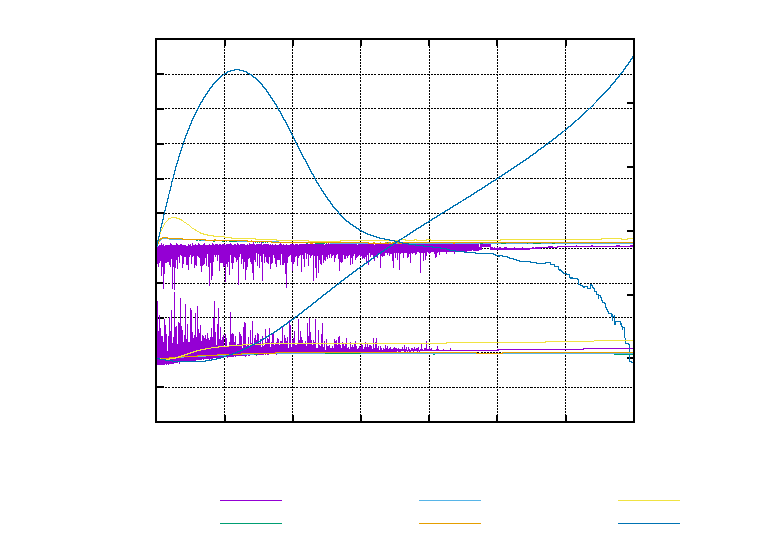
\includegraphics[width={360.00bp},height={252.00bp}]{./Vitess-contrainteDeviatorique}}%
    \gplfronttext
  \end{picture}%
\endgroup
}
                \caption{Contrainte - Déformation DEM (changer la vitesse)}
            \end{figure}
        \end{column}
        \begin{column}{0.5\textwidth}
            \begin{figure}[h]
                \centering
                \scalebox{0.5}{% GNUPLOT: LaTeX picture with Postscript
\begingroup
  \makeatletter
  \providecommand\color[2][]{%
    \GenericError{(gnuplot) \space\space\space\@spaces}{%
      Package color not loaded in conjunction with
      terminal option `colourtext'%
    }{See the gnuplot documentation for explanation.%
    }{Either use 'blacktext' in gnuplot or load the package
      color.sty in LaTeX.}%
    \renewcommand\color[2][]{}%
  }%
  \providecommand\includegraphics[2][]{%
    \GenericError{(gnuplot) \space\space\space\@spaces}{%
      Package graphicx or graphics not loaded%
    }{See the gnuplot documentation for explanation.%
    }{The gnuplot epslatex terminal needs graphicx.sty or graphics.sty.}%
    \renewcommand\includegraphics[2][]{}%
  }%
  \providecommand\rotatebox[2]{#2}%
  \@ifundefined{ifGPcolor}{%
    \newif\ifGPcolor
    \GPcolortrue
  }{}%
  \@ifundefined{ifGPblacktext}{%
    \newif\ifGPblacktext
    \GPblacktextfalse
  }{}%
  % define a \g@addto@macro without @ in the name:
  \let\gplgaddtomacro\g@addto@macro
  % define empty templates for all commands taking text:
  \gdef\gplbacktext{}%
  \gdef\gplfronttext{}%
  \makeatother
  \ifGPblacktext
    % no textcolor at all
    \def\colorrgb#1{}%
    \def\colorgray#1{}%
  \else
    % gray or color?
    \ifGPcolor
      \def\colorrgb#1{\color[rgb]{#1}}%
      \def\colorgray#1{\color[gray]{#1}}%
      \expandafter\def\csname LTw\endcsname{\color{white}}%
      \expandafter\def\csname LTb\endcsname{\color{black}}%
      \expandafter\def\csname LTa\endcsname{\color{black}}%
      \expandafter\def\csname LT0\endcsname{\color[rgb]{1,0,0}}%
      \expandafter\def\csname LT1\endcsname{\color[rgb]{0,1,0}}%
      \expandafter\def\csname LT2\endcsname{\color[rgb]{0,0,1}}%
      \expandafter\def\csname LT3\endcsname{\color[rgb]{1,0,1}}%
      \expandafter\def\csname LT4\endcsname{\color[rgb]{0,1,1}}%
      \expandafter\def\csname LT5\endcsname{\color[rgb]{1,1,0}}%
      \expandafter\def\csname LT6\endcsname{\color[rgb]{0,0,0}}%
      \expandafter\def\csname LT7\endcsname{\color[rgb]{1,0.3,0}}%
      \expandafter\def\csname LT8\endcsname{\color[rgb]{0.5,0.5,0.5}}%
    \else
      % gray
      \def\colorrgb#1{\color{black}}%
      \def\colorgray#1{\color[gray]{#1}}%
      \expandafter\def\csname LTw\endcsname{\color{white}}%
      \expandafter\def\csname LTb\endcsname{\color{black}}%
      \expandafter\def\csname LTa\endcsname{\color{black}}%
      \expandafter\def\csname LT0\endcsname{\color{black}}%
      \expandafter\def\csname LT1\endcsname{\color{black}}%
      \expandafter\def\csname LT2\endcsname{\color{black}}%
      \expandafter\def\csname LT3\endcsname{\color{black}}%
      \expandafter\def\csname LT4\endcsname{\color{black}}%
      \expandafter\def\csname LT5\endcsname{\color{black}}%
      \expandafter\def\csname LT6\endcsname{\color{black}}%
      \expandafter\def\csname LT7\endcsname{\color{black}}%
      \expandafter\def\csname LT8\endcsname{\color{black}}%
    \fi
  \fi
    \setlength{\unitlength}{0.0500bp}%
    \ifx\gptboxheight\undefined%
      \newlength{\gptboxheight}%
      \newlength{\gptboxwidth}%
      \newsavebox{\gptboxtext}%
    \fi%
    \setlength{\fboxrule}{0.5pt}%
    \setlength{\fboxsep}{1pt}%
    \definecolor{tbcol}{rgb}{1,1,1}%
\begin{picture}(7200.00,5040.00)%
    \gplgaddtomacro\gplbacktext{%
      \csname LTb\endcsname%%
      \put(814,440){\makebox(0,0)[r]{\strut{}$0$}}%
      \csname LTb\endcsname%%
      \put(814,1236){\makebox(0,0)[r]{\strut{}$100$}}%
      \csname LTb\endcsname%%
      \put(814,2032){\makebox(0,0)[r]{\strut{}$200$}}%
      \csname LTb\endcsname%%
      \put(814,2829){\makebox(0,0)[r]{\strut{}$300$}}%
      \csname LTb\endcsname%%
      \put(814,3625){\makebox(0,0)[r]{\strut{}$400$}}%
      \csname LTb\endcsname%%
      \put(814,4421){\makebox(0,0)[r]{\strut{}$500$}}%
      \csname LTb\endcsname%%
      \put(946,220){\makebox(0,0){\strut{}$0$}}%
      \csname LTb\endcsname%%
      \put(1922,220){\makebox(0,0){\strut{}$0.5$}}%
      \csname LTb\endcsname%%
      \put(2898,220){\makebox(0,0){\strut{}$1$}}%
      \csname LTb\endcsname%%
      \put(3875,220){\makebox(0,0){\strut{}$1.5$}}%
      \csname LTb\endcsname%%
      \put(4851,220){\makebox(0,0){\strut{}$2$}}%
      \csname LTb\endcsname%%
      \put(5827,220){\makebox(0,0){\strut{}$2.5$}}%
      \csname LTb\endcsname%%
      \put(6803,220){\makebox(0,0){\strut{}$3$}}%
    }%
    \gplgaddtomacro\gplfronttext{%
      \csname LTb\endcsname%%
      \put(209,2629){\rotatebox{-270}{\makebox(0,0){\strut{}$\sigma_{yy}$}}}%
      \put(3874,286){\makebox(0,0){\strut{}$\varepsilon_{yy}$ (\%)}}%
      \csname LTb\endcsname%%
      \put(4184,663){\makebox(0,0)[r]{\strut{}$v = 1 \times 10^{-3}$}}%
      \csname LTb\endcsname%%
      \put(6032,663){\makebox(0,0)[r]{\strut{}$v = 5 \times 10^{-3}$}}%
    }%
    \gplbacktext
    \put(0,0){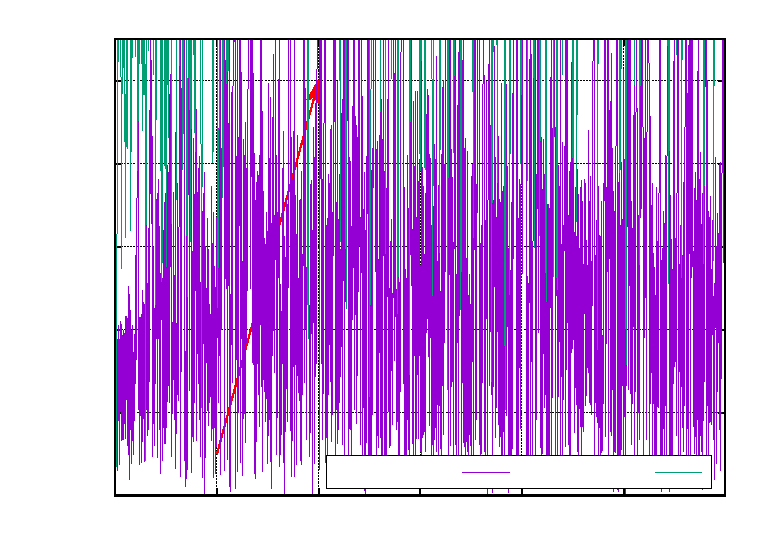
\includegraphics[width={360.00bp},height={252.00bp}]{./PasTemps}}%
    \gplfronttext
  \end{picture}%
\endgroup
}
                \caption{Bruyant concernant pas de temps MPM (avant)}
            \end{figure}
        \end{column}
    \end{columns}
    \[
        \dot{x}(t) = \frac{x(t+\varepsilon) - x(t-\varepsilon)}{2\varepsilon}
    \]
    Problème de arrondir?
\end{frame}

% \begin{frame}{Comparer entre les formes de boite}
%     \begin{columns}
%         \begin{column}{0.5\textwidth}
%             \begin{figure}[h]
%                 \centering
%                 \scalebox{0.5}{% GNUPLOT: LaTeX picture with Postscript
\begingroup
  \makeatletter
  \providecommand\color[2][]{%
    \GenericError{(gnuplot) \space\space\space\@spaces}{%
      Package color not loaded in conjunction with
      terminal option `colourtext'%
    }{See the gnuplot documentation for explanation.%
    }{Either use 'blacktext' in gnuplot or load the package
      color.sty in LaTeX.}%
    \renewcommand\color[2][]{}%
  }%
  \providecommand\includegraphics[2][]{%
    \GenericError{(gnuplot) \space\space\space\@spaces}{%
      Package graphicx or graphics not loaded%
    }{See the gnuplot documentation for explanation.%
    }{The gnuplot epslatex terminal needs graphicx.sty or graphics.sty.}%
    \renewcommand\includegraphics[2][]{}%
  }%
  \providecommand\rotatebox[2]{#2}%
  \@ifundefined{ifGPcolor}{%
    \newif\ifGPcolor
    \GPcolortrue
  }{}%
  \@ifundefined{ifGPblacktext}{%
    \newif\ifGPblacktext
    \GPblacktextfalse
  }{}%
  % define a \g@addto@macro without @ in the name:
  \let\gplgaddtomacro\g@addto@macro
  % define empty templates for all commands taking text:
  \gdef\gplbacktext{}%
  \gdef\gplfronttext{}%
  \makeatother
  \ifGPblacktext
    % no textcolor at all
    \def\colorrgb#1{}%
    \def\colorgray#1{}%
  \else
    % gray or color?
    \ifGPcolor
      \def\colorrgb#1{\color[rgb]{#1}}%
      \def\colorgray#1{\color[gray]{#1}}%
      \expandafter\def\csname LTw\endcsname{\color{white}}%
      \expandafter\def\csname LTb\endcsname{\color{black}}%
      \expandafter\def\csname LTa\endcsname{\color{black}}%
      \expandafter\def\csname LT0\endcsname{\color[rgb]{1,0,0}}%
      \expandafter\def\csname LT1\endcsname{\color[rgb]{0,1,0}}%
      \expandafter\def\csname LT2\endcsname{\color[rgb]{0,0,1}}%
      \expandafter\def\csname LT3\endcsname{\color[rgb]{1,0,1}}%
      \expandafter\def\csname LT4\endcsname{\color[rgb]{0,1,1}}%
      \expandafter\def\csname LT5\endcsname{\color[rgb]{1,1,0}}%
      \expandafter\def\csname LT6\endcsname{\color[rgb]{0,0,0}}%
      \expandafter\def\csname LT7\endcsname{\color[rgb]{1,0.3,0}}%
      \expandafter\def\csname LT8\endcsname{\color[rgb]{0.5,0.5,0.5}}%
    \else
      % gray
      \def\colorrgb#1{\color{black}}%
      \def\colorgray#1{\color[gray]{#1}}%
      \expandafter\def\csname LTw\endcsname{\color{white}}%
      \expandafter\def\csname LTb\endcsname{\color{black}}%
      \expandafter\def\csname LTa\endcsname{\color{black}}%
      \expandafter\def\csname LT0\endcsname{\color{black}}%
      \expandafter\def\csname LT1\endcsname{\color{black}}%
      \expandafter\def\csname LT2\endcsname{\color{black}}%
      \expandafter\def\csname LT3\endcsname{\color{black}}%
      \expandafter\def\csname LT4\endcsname{\color{black}}%
      \expandafter\def\csname LT5\endcsname{\color{black}}%
      \expandafter\def\csname LT6\endcsname{\color{black}}%
      \expandafter\def\csname LT7\endcsname{\color{black}}%
      \expandafter\def\csname LT8\endcsname{\color{black}}%
    \fi
  \fi
    \setlength{\unitlength}{0.0500bp}%
    \ifx\gptboxheight\undefined%
      \newlength{\gptboxheight}%
      \newlength{\gptboxwidth}%
      \newsavebox{\gptboxtext}%
    \fi%
    \setlength{\fboxrule}{0.5pt}%
    \setlength{\fboxsep}{1pt}%
    \definecolor{tbcol}{rgb}{1,1,1}%
\begin{picture}(7200.00,5040.00)%
    \gplgaddtomacro\gplbacktext{%
      \csname LTb\endcsname%%
      \put(946,1144){\makebox(0,0)[r]{\strut{}$0$}}%
      \csname LTb\endcsname%%
      \put(946,1757){\makebox(0,0)[r]{\strut{}$200$}}%
      \csname LTb\endcsname%%
      \put(946,2369){\makebox(0,0)[r]{\strut{}$400$}}%
      \csname LTb\endcsname%%
      \put(946,2982){\makebox(0,0)[r]{\strut{}$600$}}%
      \csname LTb\endcsname%%
      \put(946,3594){\makebox(0,0)[r]{\strut{}$800$}}%
      \csname LTb\endcsname%%
      \put(946,4207){\makebox(0,0)[r]{\strut{}$1000$}}%
      \csname LTb\endcsname%%
      \put(946,4819){\makebox(0,0)[r]{\strut{}$1200$}}%
      \csname LTb\endcsname%%
      \put(1078,924){\makebox(0,0){\strut{}$0$}}%
      \csname LTb\endcsname%%
      \put(1667,924){\makebox(0,0){\strut{}$10$}}%
      \csname LTb\endcsname%%
      \put(2256,924){\makebox(0,0){\strut{}$20$}}%
      \csname LTb\endcsname%%
      \put(2845,924){\makebox(0,0){\strut{}$30$}}%
      \csname LTb\endcsname%%
      \put(3435,924){\makebox(0,0){\strut{}$40$}}%
      \csname LTb\endcsname%%
      \put(4024,924){\makebox(0,0){\strut{}$50$}}%
      \csname LTb\endcsname%%
      \put(4613,924){\makebox(0,0){\strut{}$60$}}%
      \csname LTb\endcsname%%
      \put(5202,924){\makebox(0,0){\strut{}$70$}}%
      \csname LTb\endcsname%%
      \put(5791,924){\makebox(0,0){\strut{}$80$}}%
      \put(5923,1144){\makebox(0,0)[l]{\strut{}$-100$}}%
      \put(5923,1669){\makebox(0,0)[l]{\strut{}$0$}}%
      \put(5923,2194){\makebox(0,0)[l]{\strut{}$100$}}%
      \put(5923,2719){\makebox(0,0)[l]{\strut{}$200$}}%
      \put(5923,3244){\makebox(0,0)[l]{\strut{}$300$}}%
      \put(5923,3769){\makebox(0,0)[l]{\strut{}$400$}}%
      \put(5923,4294){\makebox(0,0)[l]{\strut{}$500$}}%
      \put(5923,4819){\makebox(0,0)[l]{\strut{}$600$}}%
    }%
    \gplgaddtomacro\gplfronttext{%
      \csname LTb\endcsname%%
      \put(341,2981){\rotatebox{-270}{\makebox(0,0){\strut{}q (kPa)}}}%
      \put(6693,2981){\rotatebox{-270}{\makebox(0,0){\strut{}$\varepsilon_v$ (\%)}}}%
      \put(3434,594){\makebox(0,0){\strut{}$\varepsilon_{yy}$ (\%)}}%
      \csname LTb\endcsname%%
      \put(1624,393){\makebox(0,0)[r]{\strut{}I $= 10^{-4}$}}%
      \csname LTb\endcsname%%
      \put(1624,173){\makebox(0,0)[r]{\strut{}I $= 10^{-3}$}}%
      \csname LTb\endcsname%%
      \put(3535,393){\makebox(0,0)[r]{\strut{}I $= 10^{-2}$}}%
      \csname LTb\endcsname%%
      \put(3535,173){\makebox(0,0)[r]{\strut{}I $= 10^{-1}$}}%
      \csname LTb\endcsname%%
      \put(5446,393){\makebox(0,0)[r]{\strut{}I $= 10^{-0}$}}%
    }%
    \gplbacktext
    \put(0,0){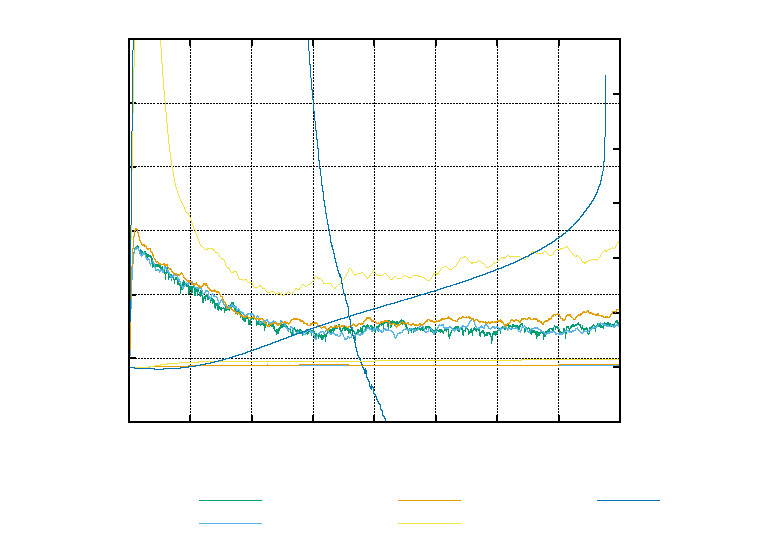
\includegraphics[width={360.00bp},height={252.00bp}]{./contrainteDeviatorique}}%
    \gplfronttext
  \end{picture}%
\endgroup
}
%                 \caption{Rectangulaire}
%             \end{figure}
%         \end{column}
%         \begin{column}{0.5\textwidth}
%             \begin{figure}[h]
%                 \centering
%                 \scalebox{0.5}{% GNUPLOT: LaTeX picture with Postscript
\begingroup
  \makeatletter
  \providecommand\color[2][]{%
    \GenericError{(gnuplot) \space\space\space\@spaces}{%
      Package color not loaded in conjunction with
      terminal option `colourtext'%
    }{See the gnuplot documentation for explanation.%
    }{Either use 'blacktext' in gnuplot or load the package
      color.sty in LaTeX.}%
    \renewcommand\color[2][]{}%
  }%
  \providecommand\includegraphics[2][]{%
    \GenericError{(gnuplot) \space\space\space\@spaces}{%
      Package graphicx or graphics not loaded%
    }{See the gnuplot documentation for explanation.%
    }{The gnuplot epslatex terminal needs graphicx.sty or graphics.sty.}%
    \renewcommand\includegraphics[2][]{}%
  }%
  \providecommand\rotatebox[2]{#2}%
  \@ifundefined{ifGPcolor}{%
    \newif\ifGPcolor
    \GPcolortrue
  }{}%
  \@ifundefined{ifGPblacktext}{%
    \newif\ifGPblacktext
    \GPblacktextfalse
  }{}%
  % define a \g@addto@macro without @ in the name:
  \let\gplgaddtomacro\g@addto@macro
  % define empty templates for all commands taking text:
  \gdef\gplbacktext{}%
  \gdef\gplfronttext{}%
  \makeatother
  \ifGPblacktext
    % no textcolor at all
    \def\colorrgb#1{}%
    \def\colorgray#1{}%
  \else
    % gray or color?
    \ifGPcolor
      \def\colorrgb#1{\color[rgb]{#1}}%
      \def\colorgray#1{\color[gray]{#1}}%
      \expandafter\def\csname LTw\endcsname{\color{white}}%
      \expandafter\def\csname LTb\endcsname{\color{black}}%
      \expandafter\def\csname LTa\endcsname{\color{black}}%
      \expandafter\def\csname LT0\endcsname{\color[rgb]{1,0,0}}%
      \expandafter\def\csname LT1\endcsname{\color[rgb]{0,1,0}}%
      \expandafter\def\csname LT2\endcsname{\color[rgb]{0,0,1}}%
      \expandafter\def\csname LT3\endcsname{\color[rgb]{1,0,1}}%
      \expandafter\def\csname LT4\endcsname{\color[rgb]{0,1,1}}%
      \expandafter\def\csname LT5\endcsname{\color[rgb]{1,1,0}}%
      \expandafter\def\csname LT6\endcsname{\color[rgb]{0,0,0}}%
      \expandafter\def\csname LT7\endcsname{\color[rgb]{1,0.3,0}}%
      \expandafter\def\csname LT8\endcsname{\color[rgb]{0.5,0.5,0.5}}%
    \else
      % gray
      \def\colorrgb#1{\color{black}}%
      \def\colorgray#1{\color[gray]{#1}}%
      \expandafter\def\csname LTw\endcsname{\color{white}}%
      \expandafter\def\csname LTb\endcsname{\color{black}}%
      \expandafter\def\csname LTa\endcsname{\color{black}}%
      \expandafter\def\csname LT0\endcsname{\color{black}}%
      \expandafter\def\csname LT1\endcsname{\color{black}}%
      \expandafter\def\csname LT2\endcsname{\color{black}}%
      \expandafter\def\csname LT3\endcsname{\color{black}}%
      \expandafter\def\csname LT4\endcsname{\color{black}}%
      \expandafter\def\csname LT5\endcsname{\color{black}}%
      \expandafter\def\csname LT6\endcsname{\color{black}}%
      \expandafter\def\csname LT7\endcsname{\color{black}}%
      \expandafter\def\csname LT8\endcsname{\color{black}}%
    \fi
  \fi
    \setlength{\unitlength}{0.0500bp}%
    \ifx\gptboxheight\undefined%
      \newlength{\gptboxheight}%
      \newlength{\gptboxwidth}%
      \newsavebox{\gptboxtext}%
    \fi%
    \setlength{\fboxrule}{0.5pt}%
    \setlength{\fboxsep}{1pt}%
    \definecolor{tbcol}{rgb}{1,1,1}%
\begin{picture}(7200.00,5040.00)%
    \gplgaddtomacro\gplbacktext{%
      \csname LTb\endcsname%%
      \put(946,1584){\makebox(0,0)[r]{\strut{}$0$}}%
      \csname LTb\endcsname%%
      \put(946,2123){\makebox(0,0)[r]{\strut{}$200$}}%
      \csname LTb\endcsname%%
      \put(946,2662){\makebox(0,0)[r]{\strut{}$400$}}%
      \csname LTb\endcsname%%
      \put(946,3202){\makebox(0,0)[r]{\strut{}$600$}}%
      \csname LTb\endcsname%%
      \put(946,3741){\makebox(0,0)[r]{\strut{}$800$}}%
      \csname LTb\endcsname%%
      \put(946,4280){\makebox(0,0)[r]{\strut{}$1000$}}%
      \csname LTb\endcsname%%
      \put(946,4819){\makebox(0,0)[r]{\strut{}$1200$}}%
      \csname LTb\endcsname%%
      \put(1078,1364){\makebox(0,0){\strut{}$0$}}%
      \csname LTb\endcsname%%
      \put(1700,1364){\makebox(0,0){\strut{}$10$}}%
      \csname LTb\endcsname%%
      \put(2322,1364){\makebox(0,0){\strut{}$20$}}%
      \csname LTb\endcsname%%
      \put(2944,1364){\makebox(0,0){\strut{}$30$}}%
      \csname LTb\endcsname%%
      \put(3567,1364){\makebox(0,0){\strut{}$40$}}%
      \csname LTb\endcsname%%
      \put(4189,1364){\makebox(0,0){\strut{}$50$}}%
      \csname LTb\endcsname%%
      \put(4811,1364){\makebox(0,0){\strut{}$60$}}%
      \csname LTb\endcsname%%
      \put(5433,1364){\makebox(0,0){\strut{}$70$}}%
      \csname LTb\endcsname%%
      \put(6055,1364){\makebox(0,0){\strut{}$80$}}%
      \put(6187,1584){\makebox(0,0)[l]{\strut{}$-2$}}%
      \put(6187,1908){\makebox(0,0)[l]{\strut{}$-1$}}%
      \put(6187,2231){\makebox(0,0)[l]{\strut{}$0$}}%
      \put(6187,2555){\makebox(0,0)[l]{\strut{}$1$}}%
      \put(6187,2878){\makebox(0,0)[l]{\strut{}$2$}}%
      \put(6187,3202){\makebox(0,0)[l]{\strut{}$3$}}%
      \put(6187,3525){\makebox(0,0)[l]{\strut{}$4$}}%
      \put(6187,3849){\makebox(0,0)[l]{\strut{}$5$}}%
      \put(6187,4172){\makebox(0,0)[l]{\strut{}$6$}}%
      \put(6187,4496){\makebox(0,0)[l]{\strut{}$7$}}%
      \put(6187,4819){\makebox(0,0)[l]{\strut{}$8$}}%
    }%
    \gplgaddtomacro\gplfronttext{%
      \csname LTb\endcsname%%
      \put(341,3201){\rotatebox{-270}{\makebox(0,0){\strut{}q (kPa)}}}%
      \put(6693,3201){\rotatebox{-270}{\makebox(0,0){\strut{}$\varepsilon_v$ (\%)}}}%
      \put(3566,1034){\makebox(0,0){\strut{}$\varepsilon_{yy}$ (\%)}}%
      \csname LTb\endcsname%%
      \put(2711,833){\makebox(0,0)[r]{\strut{}$I = 1 \times 10^{-4}$}}%
      \csname LTb\endcsname%%
      \put(2711,613){\makebox(0,0)[r]{\strut{}$I = 1 \times 10^{-3}$}}%
      \csname LTb\endcsname%%
      \put(2711,393){\makebox(0,0)[r]{\strut{}$I = 2 \times 10^{-3}$}}%
      \csname LTb\endcsname%%
      \put(2711,173){\makebox(0,0)[r]{\strut{}$I = 4 \times 10^{-3}$}}%
      \csname LTb\endcsname%%
      \put(5150,833){\makebox(0,0)[r]{\strut{}$I = 6 \times 10^{-3}$}}%
      \csname LTb\endcsname%%
      \put(5150,613){\makebox(0,0)[r]{\strut{}$I = 8 \times 10^{-3}$}}%
      \csname LTb\endcsname%%
      \put(5150,393){\makebox(0,0)[r]{\strut{}$I = 1 \times 10^{-2}$}}%
    }%
    \gplbacktext
    \put(0,0){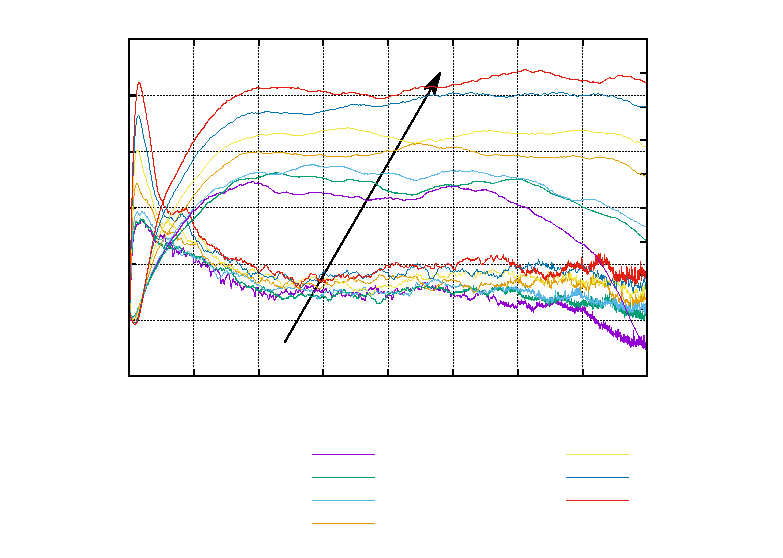
\includegraphics[width={360.00bp},height={252.00bp}]{./Test}}%
    \gplfronttext
  \end{picture}%
\endgroup
}
%                 \caption{Cube (précédent)}
%             \end{figure}
%         \end{column}
%     \end{columns}
%     En compression quasi-statique, la contrainte déviatorique au pic ou à l’état critique (donc  $\mu$) ne présente aucune différence entre les deux formes.
% \end{frame}



\begin{frame}{Problème d'arrondir (Standard IEEE 754)}
    \begin{itemize}
        \item Un type flottant ne représente qu’un nombre limité de chiffres significatifs ; au-delà, la valeur devient inexacte.
        \item Manipulation délicate à cause des différences entre binaire et décimal.
        \item Les opérations mathématiques amplifient les erreurs d’arrondi (e.g: $+$ et $\times$).
    \end{itemize}
    \begin{figure}[h]
        \centering
        \scalebox{0.15}{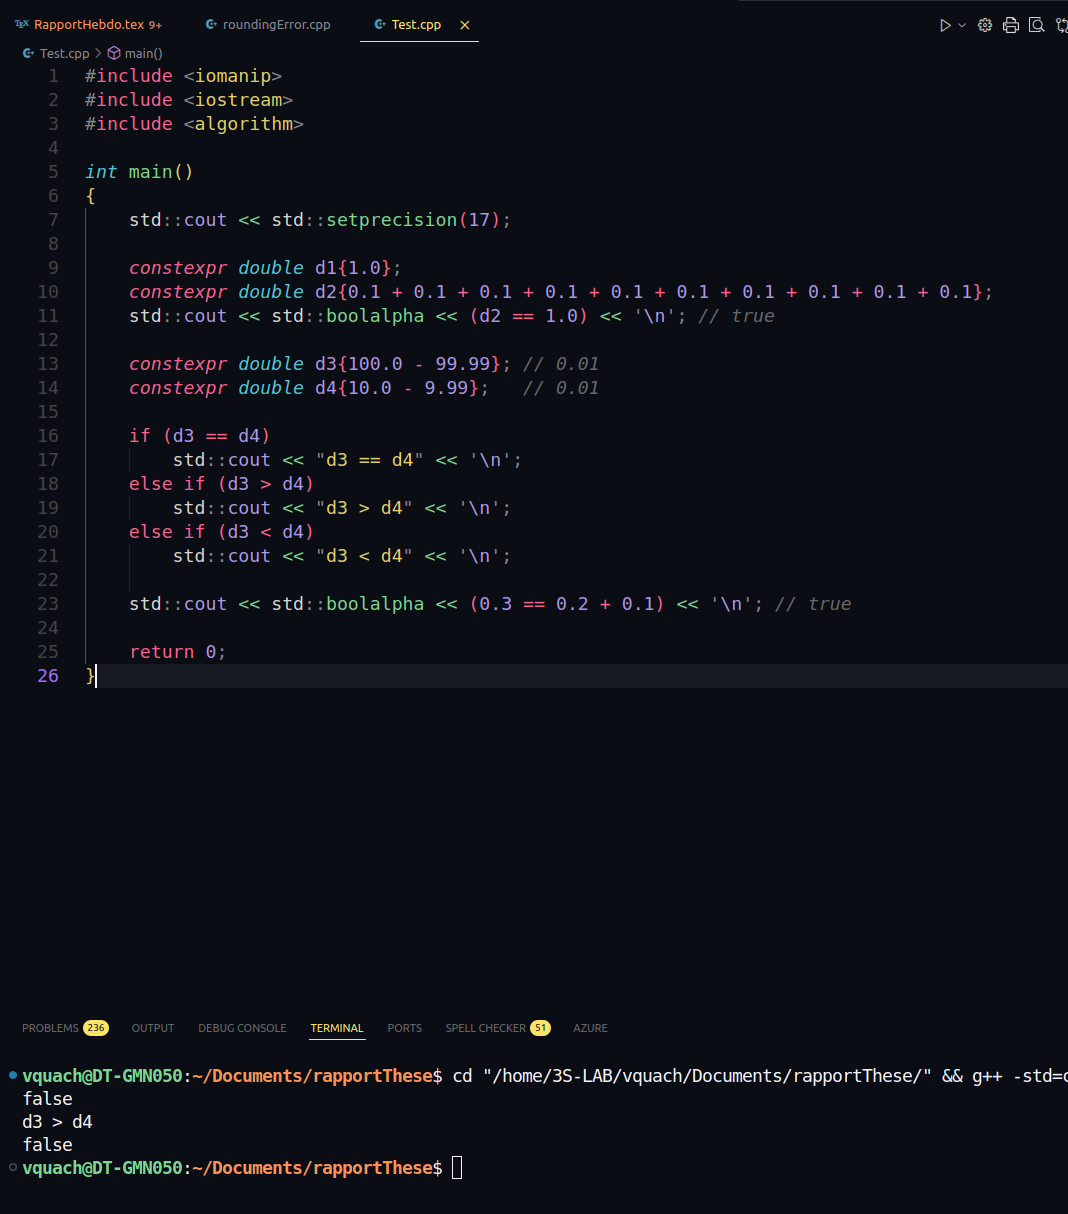
\includegraphics{pbArrondir.png}}
        \caption{La programme}
    \end{figure}
\end{frame}






\begin{frame}{Revient chez DEM - cellule cube}
    \begin{center}
        \scalebox{0.8}{\animategraphics[autoplay,loop,width=0.7\textwidth]{3}{box}{1}{3}}
    \end{center}
\end{frame}

\begin{frame}{Problème d'arrondir (Standard IEEE 754)}
    \begin{itemize}
        \item The Art of Computer Programming, Volume II: Seminumerical Algorithms (Addison-Wesley, 1969)”
        \item Toujours contrôler la tolérance d’erreur ($\epsilon$) au lieu de compter sur la “précision absolue” de l’ordinateur.
    \end{itemize}
    \begin{figure}[h]
        \centering
        \scalebox{0.14}{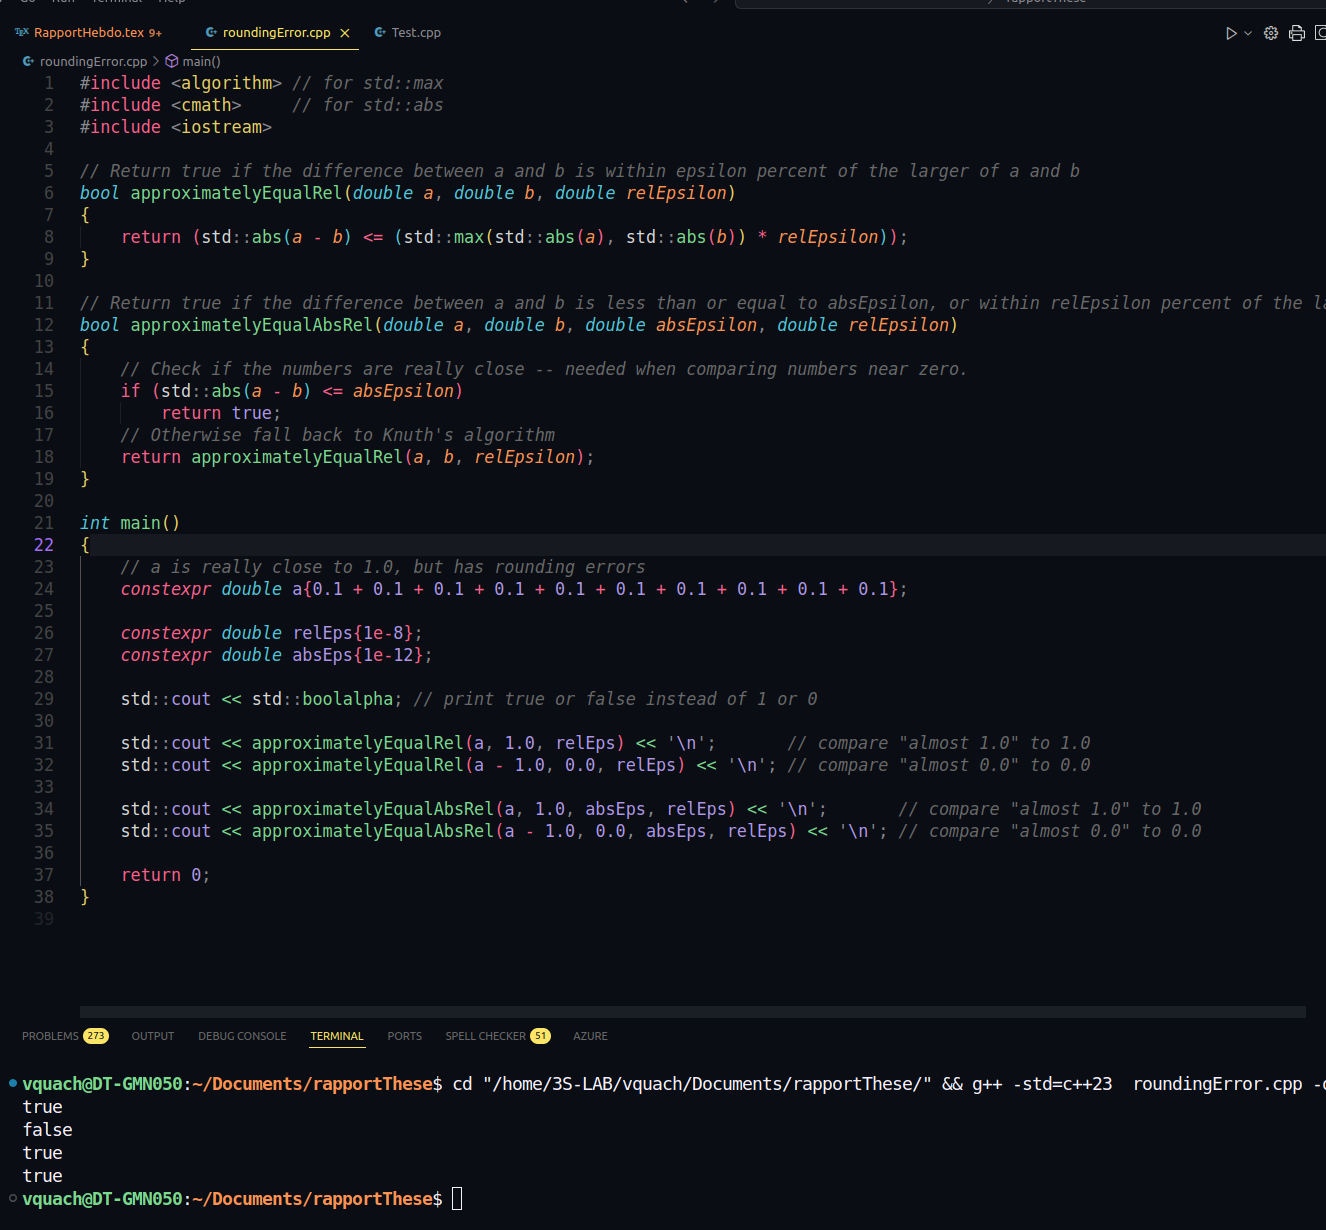
\includegraphics{solutionPbArrondir.png}}
        \caption{Fonction de comparison}
    \end{figure}
\end{frame}


\begin{frame}{Code : ajouter tous les parties dynamiques}
    \begin{figure}[h]
        \centering
        \scalebox{0.5}{% GNUPLOT: LaTeX picture with Postscript
\begingroup
  \makeatletter
  \providecommand\color[2][]{%
    \GenericError{(gnuplot) \space\space\space\@spaces}{%
      Package color not loaded in conjunction with
      terminal option `colourtext'%
    }{See the gnuplot documentation for explanation.%
    }{Either use 'blacktext' in gnuplot or load the package
      color.sty in LaTeX.}%
    \renewcommand\color[2][]{}%
  }%
  \providecommand\includegraphics[2][]{%
    \GenericError{(gnuplot) \space\space\space\@spaces}{%
      Package graphicx or graphics not loaded%
    }{See the gnuplot documentation for explanation.%
    }{The gnuplot epslatex terminal needs graphicx.sty or graphics.sty.}%
    \renewcommand\includegraphics[2][]{}%
  }%
  \providecommand\rotatebox[2]{#2}%
  \@ifundefined{ifGPcolor}{%
    \newif\ifGPcolor
    \GPcolortrue
  }{}%
  \@ifundefined{ifGPblacktext}{%
    \newif\ifGPblacktext
    \GPblacktextfalse
  }{}%
  % define a \g@addto@macro without @ in the name:
  \let\gplgaddtomacro\g@addto@macro
  % define empty templates for all commands taking text:
  \gdef\gplbacktext{}%
  \gdef\gplfronttext{}%
  \makeatother
  \ifGPblacktext
    % no textcolor at all
    \def\colorrgb#1{}%
    \def\colorgray#1{}%
  \else
    % gray or color?
    \ifGPcolor
      \def\colorrgb#1{\color[rgb]{#1}}%
      \def\colorgray#1{\color[gray]{#1}}%
      \expandafter\def\csname LTw\endcsname{\color{white}}%
      \expandafter\def\csname LTb\endcsname{\color{black}}%
      \expandafter\def\csname LTa\endcsname{\color{black}}%
      \expandafter\def\csname LT0\endcsname{\color[rgb]{1,0,0}}%
      \expandafter\def\csname LT1\endcsname{\color[rgb]{0,1,0}}%
      \expandafter\def\csname LT2\endcsname{\color[rgb]{0,0,1}}%
      \expandafter\def\csname LT3\endcsname{\color[rgb]{1,0,1}}%
      \expandafter\def\csname LT4\endcsname{\color[rgb]{0,1,1}}%
      \expandafter\def\csname LT5\endcsname{\color[rgb]{1,1,0}}%
      \expandafter\def\csname LT6\endcsname{\color[rgb]{0,0,0}}%
      \expandafter\def\csname LT7\endcsname{\color[rgb]{1,0.3,0}}%
      \expandafter\def\csname LT8\endcsname{\color[rgb]{0.5,0.5,0.5}}%
    \else
      % gray
      \def\colorrgb#1{\color{black}}%
      \def\colorgray#1{\color[gray]{#1}}%
      \expandafter\def\csname LTw\endcsname{\color{white}}%
      \expandafter\def\csname LTb\endcsname{\color{black}}%
      \expandafter\def\csname LTa\endcsname{\color{black}}%
      \expandafter\def\csname LT0\endcsname{\color{black}}%
      \expandafter\def\csname LT1\endcsname{\color{black}}%
      \expandafter\def\csname LT2\endcsname{\color{black}}%
      \expandafter\def\csname LT3\endcsname{\color{black}}%
      \expandafter\def\csname LT4\endcsname{\color{black}}%
      \expandafter\def\csname LT5\endcsname{\color{black}}%
      \expandafter\def\csname LT6\endcsname{\color{black}}%
      \expandafter\def\csname LT7\endcsname{\color{black}}%
      \expandafter\def\csname LT8\endcsname{\color{black}}%
    \fi
  \fi
    \setlength{\unitlength}{0.0500bp}%
    \ifx\gptboxheight\undefined%
      \newlength{\gptboxheight}%
      \newlength{\gptboxwidth}%
      \newsavebox{\gptboxtext}%
    \fi%
    \setlength{\fboxrule}{0.5pt}%
    \setlength{\fboxsep}{1pt}%
    \definecolor{tbcol}{rgb}{1,1,1}%
\begin{picture}(7200.00,5040.00)%
    \gplgaddtomacro\gplbacktext{%
      \csname LTb\endcsname%%
      \put(946,1144){\makebox(0,0)[r]{\strut{}$-100$}}%
      \csname LTb\endcsname%%
      \put(946,1603){\makebox(0,0)[r]{\strut{}$0$}}%
      \csname LTb\endcsname%%
      \put(946,2063){\makebox(0,0)[r]{\strut{}$100$}}%
      \csname LTb\endcsname%%
      \put(946,2522){\makebox(0,0)[r]{\strut{}$200$}}%
      \csname LTb\endcsname%%
      \put(946,2982){\makebox(0,0)[r]{\strut{}$300$}}%
      \csname LTb\endcsname%%
      \put(946,3441){\makebox(0,0)[r]{\strut{}$400$}}%
      \csname LTb\endcsname%%
      \put(946,3900){\makebox(0,0)[r]{\strut{}$500$}}%
      \csname LTb\endcsname%%
      \put(946,4360){\makebox(0,0)[r]{\strut{}$600$}}%
      \csname LTb\endcsname%%
      \put(946,4819){\makebox(0,0)[r]{\strut{}$700$}}%
      \csname LTb\endcsname%%
      \put(1078,924){\makebox(0,0){\strut{}$0$}}%
      \csname LTb\endcsname%%
      \put(1896,924){\makebox(0,0){\strut{}$10$}}%
      \csname LTb\endcsname%%
      \put(2714,924){\makebox(0,0){\strut{}$20$}}%
      \csname LTb\endcsname%%
      \put(3532,924){\makebox(0,0){\strut{}$30$}}%
      \csname LTb\endcsname%%
      \put(4349,924){\makebox(0,0){\strut{}$40$}}%
      \csname LTb\endcsname%%
      \put(5167,924){\makebox(0,0){\strut{}$50$}}%
      \csname LTb\endcsname%%
      \put(5985,924){\makebox(0,0){\strut{}$60$}}%
      \csname LTb\endcsname%%
      \put(6803,924){\makebox(0,0){\strut{}$70$}}%
    }%
    \gplgaddtomacro\gplfronttext{%
      \csname LTb\endcsname%%
      \put(341,2981){\rotatebox{-270}{\makebox(0,0){\strut{}q (kPa)}}}%
      \put(3940,594){\makebox(0,0){\strut{}$\l_{yy}$ (\%)}}%
      \csname LTb\endcsname%%
      \put(3085,393){\makebox(0,0)[r]{\strut{}$I = 10^{-4}$}}%
      \csname LTb\endcsname%%
      \put(3085,173){\makebox(0,0)[r]{\strut{}$I = 10^{-3}$}}%
      \csname LTb\endcsname%%
      \put(4996,393){\makebox(0,0)[r]{\strut{}$I = 10^{-2}$}}%
      \csname LTb\endcsname%%
      \put(4996,173){\makebox(0,0)[r]{\strut{}$I = 10^{-1}$}}%
    }%
    \gplbacktext
    \put(0,0){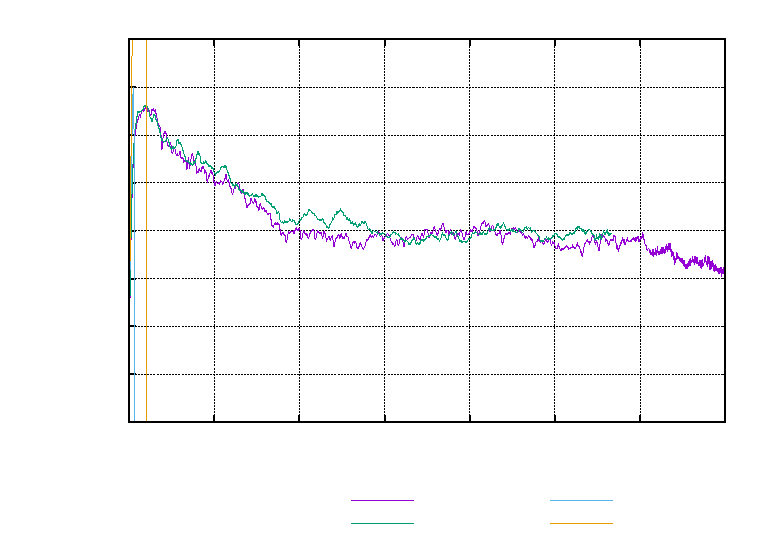
\includegraphics[width={360.00bp},height={252.00bp}]{./2termsVersion}}%
    \gplfronttext
  \end{picture}%
\endgroup
}
        \caption{Courbe Contrainte ($\sigma_3 = 300kPa$)}
    \end{figure}
    \begin{itemize}
        \item $I$ dans le régime quasi-statique : normal
        \item $I > 10^{-2}$ : calcul erroné
    \end{itemize}
    $\Rightarrow$ Les résultats varient de manière très sensible avec I
\end{frame}

\begin{frame}{Comparer entre les versions du code}
    \begin{figure}[h]
        \centering
        \scalebox{0.5}{% GNUPLOT: LaTeX picture with Postscript
\begingroup
  \makeatletter
  \providecommand\color[2][]{%
    \GenericError{(gnuplot) \space\space\space\@spaces}{%
      Package color not loaded in conjunction with
      terminal option `colourtext'%
    }{See the gnuplot documentation for explanation.%
    }{Either use 'blacktext' in gnuplot or load the package
      color.sty in LaTeX.}%
    \renewcommand\color[2][]{}%
  }%
  \providecommand\includegraphics[2][]{%
    \GenericError{(gnuplot) \space\space\space\@spaces}{%
      Package graphicx or graphics not loaded%
    }{See the gnuplot documentation for explanation.%
    }{The gnuplot epslatex terminal needs graphicx.sty or graphics.sty.}%
    \renewcommand\includegraphics[2][]{}%
  }%
  \providecommand\rotatebox[2]{#2}%
  \@ifundefined{ifGPcolor}{%
    \newif\ifGPcolor
    \GPcolortrue
  }{}%
  \@ifundefined{ifGPblacktext}{%
    \newif\ifGPblacktext
    \GPblacktextfalse
  }{}%
  % define a \g@addto@macro without @ in the name:
  \let\gplgaddtomacro\g@addto@macro
  % define empty templates for all commands taking text:
  \gdef\gplbacktext{}%
  \gdef\gplfronttext{}%
  \makeatother
  \ifGPblacktext
    % no textcolor at all
    \def\colorrgb#1{}%
    \def\colorgray#1{}%
  \else
    % gray or color?
    \ifGPcolor
      \def\colorrgb#1{\color[rgb]{#1}}%
      \def\colorgray#1{\color[gray]{#1}}%
      \expandafter\def\csname LTw\endcsname{\color{white}}%
      \expandafter\def\csname LTb\endcsname{\color{black}}%
      \expandafter\def\csname LTa\endcsname{\color{black}}%
      \expandafter\def\csname LT0\endcsname{\color[rgb]{1,0,0}}%
      \expandafter\def\csname LT1\endcsname{\color[rgb]{0,1,0}}%
      \expandafter\def\csname LT2\endcsname{\color[rgb]{0,0,1}}%
      \expandafter\def\csname LT3\endcsname{\color[rgb]{1,0,1}}%
      \expandafter\def\csname LT4\endcsname{\color[rgb]{0,1,1}}%
      \expandafter\def\csname LT5\endcsname{\color[rgb]{1,1,0}}%
      \expandafter\def\csname LT6\endcsname{\color[rgb]{0,0,0}}%
      \expandafter\def\csname LT7\endcsname{\color[rgb]{1,0.3,0}}%
      \expandafter\def\csname LT8\endcsname{\color[rgb]{0.5,0.5,0.5}}%
    \else
      % gray
      \def\colorrgb#1{\color{black}}%
      \def\colorgray#1{\color[gray]{#1}}%
      \expandafter\def\csname LTw\endcsname{\color{white}}%
      \expandafter\def\csname LTb\endcsname{\color{black}}%
      \expandafter\def\csname LTa\endcsname{\color{black}}%
      \expandafter\def\csname LT0\endcsname{\color{black}}%
      \expandafter\def\csname LT1\endcsname{\color{black}}%
      \expandafter\def\csname LT2\endcsname{\color{black}}%
      \expandafter\def\csname LT3\endcsname{\color{black}}%
      \expandafter\def\csname LT4\endcsname{\color{black}}%
      \expandafter\def\csname LT5\endcsname{\color{black}}%
      \expandafter\def\csname LT6\endcsname{\color{black}}%
      \expandafter\def\csname LT7\endcsname{\color{black}}%
      \expandafter\def\csname LT8\endcsname{\color{black}}%
    \fi
  \fi
    \setlength{\unitlength}{0.0500bp}%
    \ifx\gptboxheight\undefined%
      \newlength{\gptboxheight}%
      \newlength{\gptboxwidth}%
      \newsavebox{\gptboxtext}%
    \fi%
    \setlength{\fboxrule}{0.5pt}%
    \setlength{\fboxsep}{1pt}%
    \definecolor{tbcol}{rgb}{1,1,1}%
\begin{picture}(7200.00,5040.00)%
    \gplgaddtomacro\gplbacktext{%
      \csname LTb\endcsname%%
      \put(946,2459){\makebox(0,0)[r]{\strut{}$0$}}%
      \csname LTb\endcsname%%
      \put(946,2888){\makebox(0,0)[r]{\strut{}$200$}}%
      \csname LTb\endcsname%%
      \put(946,3317){\makebox(0,0)[r]{\strut{}$400$}}%
      \csname LTb\endcsname%%
      \put(946,3746){\makebox(0,0)[r]{\strut{}$600$}}%
      \csname LTb\endcsname%%
      \put(946,4175){\makebox(0,0)[r]{\strut{}$800$}}%
      \csname LTb\endcsname%%
      \put(946,4604){\makebox(0,0)[r]{\strut{}$1000$}}%
      \csname LTb\endcsname%%
      \put(1078,2024){\makebox(0,0){\strut{}$0$}}%
      \csname LTb\endcsname%%
      \put(1896,2024){\makebox(0,0){\strut{}$10$}}%
      \csname LTb\endcsname%%
      \put(2714,2024){\makebox(0,0){\strut{}$20$}}%
      \csname LTb\endcsname%%
      \put(3532,2024){\makebox(0,0){\strut{}$30$}}%
      \csname LTb\endcsname%%
      \put(4349,2024){\makebox(0,0){\strut{}$40$}}%
      \csname LTb\endcsname%%
      \put(5167,2024){\makebox(0,0){\strut{}$50$}}%
      \csname LTb\endcsname%%
      \put(5985,2024){\makebox(0,0){\strut{}$60$}}%
      \csname LTb\endcsname%%
      \put(6803,2024){\makebox(0,0){\strut{}$70$}}%
    }%
    \gplgaddtomacro\gplfronttext{%
      \csname LTb\endcsname%%
      \put(341,3531){\rotatebox{-270}{\makebox(0,0){\strut{}q (kPa)}}}%
      \put(3940,1694){\makebox(0,0){\strut{}$\varepsilon_{yy}$ (\%)}}%
      \csname LTb\endcsname%%
      \put(4899,1493){\makebox(0,0)[r]{\strut{}$I = 10^{-4}$ 0 terme}}%
      \csname LTb\endcsname%%
      \put(4899,1273){\makebox(0,0)[r]{\strut{}$I = 10^{-4}$ 1 terme}}%
      \csname LTb\endcsname%%
      \put(4899,1053){\makebox(0,0)[r]{\strut{}$I = 10^{-4}$ 2 termes}}%
      \csname LTb\endcsname%%
      \put(4899,833){\makebox(0,0)[r]{\strut{}$I = 10^{-2}$ 0 terme}}%
      \csname LTb\endcsname%%
      \put(4899,613){\makebox(0,0)[r]{\strut{}$I = 10^{-2}$ 1 terme}}%
      \csname LTb\endcsname%%
      \put(4899,393){\makebox(0,0)[r]{\strut{}$I = 10^{-2}$ 2 termes}}%
      \csname LTb\endcsname%%
      \put(4899,173){\makebox(0,0)[r]{\strut{}$I = 10^{-2}$ 2 termes MAJ}}%
    }%
    \gplbacktext
    \put(0,0){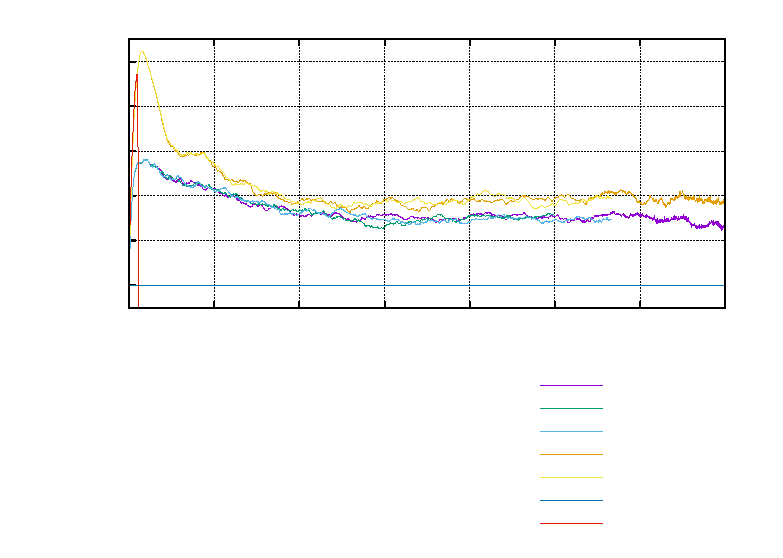
\includegraphics[width={360.00bp},height={252.00bp}]{./Synthese}}%
    \gplfronttext
  \end{picture}%
\endgroup
}
        \caption{Courbe Contrainte ($\sigma_3 = 300kPa$)}
    \end{figure}
    \begin{itemize}
        \item 0 terme : $\ddot{s} = h^{-1} \cdot (F/m)$ $\rightarrow$ ancienne version
        \item 1 terme : $\ddot{s} = h^{-1} \cdot (F/m - 2 \dot{h} \dot{r})$ $\rightarrow$ presque inchangé
        \item 2 termes : $\ddot{s} = h^{-1} \cdot (F/m - 2 \dot{h} \dot{r} - \ddot{h} r)$ $\rightarrow$ calcul erroné
    \end{itemize}
\end{frame}

\begin{frame}{Essayer de changer la masse de la périodic}
    \begin{figure}[h]
        \centering
        \scalebox{0.5}{% GNUPLOT: LaTeX picture with Postscript
\begingroup
  \makeatletter
  \providecommand\color[2][]{%
    \GenericError{(gnuplot) \space\space\space\@spaces}{%
      Package color not loaded in conjunction with
      terminal option `colourtext'%
    }{See the gnuplot documentation for explanation.%
    }{Either use 'blacktext' in gnuplot or load the package
      color.sty in LaTeX.}%
    \renewcommand\color[2][]{}%
  }%
  \providecommand\includegraphics[2][]{%
    \GenericError{(gnuplot) \space\space\space\@spaces}{%
      Package graphicx or graphics not loaded%
    }{See the gnuplot documentation for explanation.%
    }{The gnuplot epslatex terminal needs graphicx.sty or graphics.sty.}%
    \renewcommand\includegraphics[2][]{}%
  }%
  \providecommand\rotatebox[2]{#2}%
  \@ifundefined{ifGPcolor}{%
    \newif\ifGPcolor
    \GPcolortrue
  }{}%
  \@ifundefined{ifGPblacktext}{%
    \newif\ifGPblacktext
    \GPblacktextfalse
  }{}%
  % define a \g@addto@macro without @ in the name:
  \let\gplgaddtomacro\g@addto@macro
  % define empty templates for all commands taking text:
  \gdef\gplbacktext{}%
  \gdef\gplfronttext{}%
  \makeatother
  \ifGPblacktext
    % no textcolor at all
    \def\colorrgb#1{}%
    \def\colorgray#1{}%
  \else
    % gray or color?
    \ifGPcolor
      \def\colorrgb#1{\color[rgb]{#1}}%
      \def\colorgray#1{\color[gray]{#1}}%
      \expandafter\def\csname LTw\endcsname{\color{white}}%
      \expandafter\def\csname LTb\endcsname{\color{black}}%
      \expandafter\def\csname LTa\endcsname{\color{black}}%
      \expandafter\def\csname LT0\endcsname{\color[rgb]{1,0,0}}%
      \expandafter\def\csname LT1\endcsname{\color[rgb]{0,1,0}}%
      \expandafter\def\csname LT2\endcsname{\color[rgb]{0,0,1}}%
      \expandafter\def\csname LT3\endcsname{\color[rgb]{1,0,1}}%
      \expandafter\def\csname LT4\endcsname{\color[rgb]{0,1,1}}%
      \expandafter\def\csname LT5\endcsname{\color[rgb]{1,1,0}}%
      \expandafter\def\csname LT6\endcsname{\color[rgb]{0,0,0}}%
      \expandafter\def\csname LT7\endcsname{\color[rgb]{1,0.3,0}}%
      \expandafter\def\csname LT8\endcsname{\color[rgb]{0.5,0.5,0.5}}%
    \else
      % gray
      \def\colorrgb#1{\color{black}}%
      \def\colorgray#1{\color[gray]{#1}}%
      \expandafter\def\csname LTw\endcsname{\color{white}}%
      \expandafter\def\csname LTb\endcsname{\color{black}}%
      \expandafter\def\csname LTa\endcsname{\color{black}}%
      \expandafter\def\csname LT0\endcsname{\color{black}}%
      \expandafter\def\csname LT1\endcsname{\color{black}}%
      \expandafter\def\csname LT2\endcsname{\color{black}}%
      \expandafter\def\csname LT3\endcsname{\color{black}}%
      \expandafter\def\csname LT4\endcsname{\color{black}}%
      \expandafter\def\csname LT5\endcsname{\color{black}}%
      \expandafter\def\csname LT6\endcsname{\color{black}}%
      \expandafter\def\csname LT7\endcsname{\color{black}}%
      \expandafter\def\csname LT8\endcsname{\color{black}}%
    \fi
  \fi
    \setlength{\unitlength}{0.0500bp}%
    \ifx\gptboxheight\undefined%
      \newlength{\gptboxheight}%
      \newlength{\gptboxwidth}%
      \newsavebox{\gptboxtext}%
    \fi%
    \setlength{\fboxrule}{0.5pt}%
    \setlength{\fboxsep}{1pt}%
    \definecolor{tbcol}{rgb}{1,1,1}%
\begin{picture}(7200.00,5040.00)%
    \gplgaddtomacro\gplbacktext{%
      \csname LTb\endcsname%%
      \put(1078,1144){\makebox(0,0)[r]{\strut{}$-1000$}}%
      \csname LTb\endcsname%%
      \put(1078,1669){\makebox(0,0)[r]{\strut{}$0$}}%
      \csname LTb\endcsname%%
      \put(1078,2194){\makebox(0,0)[r]{\strut{}$1000$}}%
      \csname LTb\endcsname%%
      \put(1078,2719){\makebox(0,0)[r]{\strut{}$2000$}}%
      \csname LTb\endcsname%%
      \put(1078,3244){\makebox(0,0)[r]{\strut{}$3000$}}%
      \csname LTb\endcsname%%
      \put(1078,3769){\makebox(0,0)[r]{\strut{}$4000$}}%
      \csname LTb\endcsname%%
      \put(1078,4294){\makebox(0,0)[r]{\strut{}$5000$}}%
      \csname LTb\endcsname%%
      \put(1078,4819){\makebox(0,0)[r]{\strut{}$6000$}}%
      \csname LTb\endcsname%%
      \put(1210,924){\makebox(0,0){\strut{}$0$}}%
      \csname LTb\endcsname%%
      \put(2009,924){\makebox(0,0){\strut{}$10$}}%
      \csname LTb\endcsname%%
      \put(2808,924){\makebox(0,0){\strut{}$20$}}%
      \csname LTb\endcsname%%
      \put(3607,924){\makebox(0,0){\strut{}$30$}}%
      \csname LTb\endcsname%%
      \put(4406,924){\makebox(0,0){\strut{}$40$}}%
      \csname LTb\endcsname%%
      \put(5205,924){\makebox(0,0){\strut{}$50$}}%
      \csname LTb\endcsname%%
      \put(6004,924){\makebox(0,0){\strut{}$60$}}%
      \csname LTb\endcsname%%
      \put(6803,924){\makebox(0,0){\strut{}$70$}}%
    }%
    \gplgaddtomacro\gplfronttext{%
      \csname LTb\endcsname%%
      \put(341,2981){\rotatebox{-270}{\makebox(0,0){\strut{}q (kPa)}}}%
      \put(4006,594){\makebox(0,0){\strut{}$\varepsilon_{yy}$ (\%)}}%
      \csname LTb\endcsname%%
      \put(3151,393){\makebox(0,0)[r]{\strut{}une particule}}%
      \csname LTb\endcsname%%
      \put(3151,173){\makebox(0,0)[r]{\strut{}une tranche}}%
      \csname LTb\endcsname%%
      \put(5722,393){\makebox(0,0)[r]{\strut{}masse totale}}%
    }%
    \gplbacktext
    \put(0,0){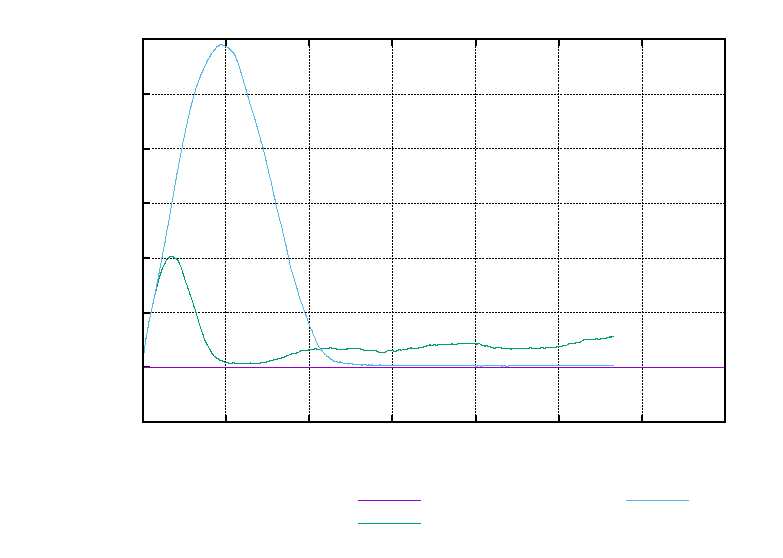
\includegraphics[width={360.00bp},height={252.00bp}]{./Masse}}%
    \gplfronttext
  \end{picture}%
\endgroup
}
        \caption{Courbe Contrainte ($I = 10^{-2}$)}
    \end{figure}
    \[
        \ddot{h}_{xx} = \frac{V_{\text{cell}} \, (\sigma_{xx} - p)}{h_{xx} \, h_{\text{mass}}}
    \]
    \[
        \ddot{h}_{yy} = \frac{V_{\text{cell}} \, (\sigma_{yy} - p)}{h_{yy} \, h_{\text{mass}}}
    \]

\end{frame}

\begin{frame}{Les résultats varient de manière très sensible avec $I$}
    \begin{figure}[h]
        \centering
        \scalebox{0.5}{% GNUPLOT: LaTeX picture with Postscript
\begingroup
  \makeatletter
  \providecommand\color[2][]{%
    \GenericError{(gnuplot) \space\space\space\@spaces}{%
      Package color not loaded in conjunction with
      terminal option `colourtext'%
    }{See the gnuplot documentation for explanation.%
    }{Either use 'blacktext' in gnuplot or load the package
      color.sty in LaTeX.}%
    \renewcommand\color[2][]{}%
  }%
  \providecommand\includegraphics[2][]{%
    \GenericError{(gnuplot) \space\space\space\@spaces}{%
      Package graphicx or graphics not loaded%
    }{See the gnuplot documentation for explanation.%
    }{The gnuplot epslatex terminal needs graphicx.sty or graphics.sty.}%
    \renewcommand\includegraphics[2][]{}%
  }%
  \providecommand\rotatebox[2]{#2}%
  \@ifundefined{ifGPcolor}{%
    \newif\ifGPcolor
    \GPcolortrue
  }{}%
  \@ifundefined{ifGPblacktext}{%
    \newif\ifGPblacktext
    \GPblacktextfalse
  }{}%
  % define a \g@addto@macro without @ in the name:
  \let\gplgaddtomacro\g@addto@macro
  % define empty templates for all commands taking text:
  \gdef\gplbacktext{}%
  \gdef\gplfronttext{}%
  \makeatother
  \ifGPblacktext
    % no textcolor at all
    \def\colorrgb#1{}%
    \def\colorgray#1{}%
  \else
    % gray or color?
    \ifGPcolor
      \def\colorrgb#1{\color[rgb]{#1}}%
      \def\colorgray#1{\color[gray]{#1}}%
      \expandafter\def\csname LTw\endcsname{\color{white}}%
      \expandafter\def\csname LTb\endcsname{\color{black}}%
      \expandafter\def\csname LTa\endcsname{\color{black}}%
      \expandafter\def\csname LT0\endcsname{\color[rgb]{1,0,0}}%
      \expandafter\def\csname LT1\endcsname{\color[rgb]{0,1,0}}%
      \expandafter\def\csname LT2\endcsname{\color[rgb]{0,0,1}}%
      \expandafter\def\csname LT3\endcsname{\color[rgb]{1,0,1}}%
      \expandafter\def\csname LT4\endcsname{\color[rgb]{0,1,1}}%
      \expandafter\def\csname LT5\endcsname{\color[rgb]{1,1,0}}%
      \expandafter\def\csname LT6\endcsname{\color[rgb]{0,0,0}}%
      \expandafter\def\csname LT7\endcsname{\color[rgb]{1,0.3,0}}%
      \expandafter\def\csname LT8\endcsname{\color[rgb]{0.5,0.5,0.5}}%
    \else
      % gray
      \def\colorrgb#1{\color{black}}%
      \def\colorgray#1{\color[gray]{#1}}%
      \expandafter\def\csname LTw\endcsname{\color{white}}%
      \expandafter\def\csname LTb\endcsname{\color{black}}%
      \expandafter\def\csname LTa\endcsname{\color{black}}%
      \expandafter\def\csname LT0\endcsname{\color{black}}%
      \expandafter\def\csname LT1\endcsname{\color{black}}%
      \expandafter\def\csname LT2\endcsname{\color{black}}%
      \expandafter\def\csname LT3\endcsname{\color{black}}%
      \expandafter\def\csname LT4\endcsname{\color{black}}%
      \expandafter\def\csname LT5\endcsname{\color{black}}%
      \expandafter\def\csname LT6\endcsname{\color{black}}%
      \expandafter\def\csname LT7\endcsname{\color{black}}%
      \expandafter\def\csname LT8\endcsname{\color{black}}%
    \fi
  \fi
    \setlength{\unitlength}{0.0500bp}%
    \ifx\gptboxheight\undefined%
      \newlength{\gptboxheight}%
      \newlength{\gptboxwidth}%
      \newsavebox{\gptboxtext}%
    \fi%
    \setlength{\fboxrule}{0.5pt}%
    \setlength{\fboxsep}{1pt}%
    \definecolor{tbcol}{rgb}{1,1,1}%
\begin{picture}(7200.00,5040.00)%
    \gplgaddtomacro\gplbacktext{%
      \csname LTb\endcsname%%
      \put(946,1144){\makebox(0,0)[r]{\strut{}$-100$}}%
      \csname LTb\endcsname%%
      \put(946,1669){\makebox(0,0)[r]{\strut{}$0$}}%
      \csname LTb\endcsname%%
      \put(946,2194){\makebox(0,0)[r]{\strut{}$100$}}%
      \csname LTb\endcsname%%
      \put(946,2719){\makebox(0,0)[r]{\strut{}$200$}}%
      \csname LTb\endcsname%%
      \put(946,3244){\makebox(0,0)[r]{\strut{}$300$}}%
      \csname LTb\endcsname%%
      \put(946,3769){\makebox(0,0)[r]{\strut{}$400$}}%
      \csname LTb\endcsname%%
      \put(946,4294){\makebox(0,0)[r]{\strut{}$500$}}%
      \csname LTb\endcsname%%
      \put(946,4819){\makebox(0,0)[r]{\strut{}$600$}}%
      \csname LTb\endcsname%%
      \put(1078,924){\makebox(0,0){\strut{}$0$}}%
      \csname LTb\endcsname%%
      \put(1896,924){\makebox(0,0){\strut{}$10$}}%
      \csname LTb\endcsname%%
      \put(2714,924){\makebox(0,0){\strut{}$20$}}%
      \csname LTb\endcsname%%
      \put(3532,924){\makebox(0,0){\strut{}$30$}}%
      \csname LTb\endcsname%%
      \put(4349,924){\makebox(0,0){\strut{}$40$}}%
      \csname LTb\endcsname%%
      \put(5167,924){\makebox(0,0){\strut{}$50$}}%
      \csname LTb\endcsname%%
      \put(5985,924){\makebox(0,0){\strut{}$60$}}%
      \csname LTb\endcsname%%
      \put(6803,924){\makebox(0,0){\strut{}$70$}}%
    }%
    \gplgaddtomacro\gplfronttext{%
      \csname LTb\endcsname%%
      \put(341,2981){\rotatebox{-270}{\makebox(0,0){\strut{}q (kPa)}}}%
      \put(3940,594){\makebox(0,0){\strut{}$\varepsilon_{yy}$ (\%)}}%
      \csname LTb\endcsname%%
      \put(3085,393){\makebox(0,0)[r]{\strut{}$I = 4.4 \times 10^{-4}$}}%
      \csname LTb\endcsname%%
      \put(3085,173){\makebox(0,0)[r]{\strut{}$I = 4.4 \times 10^{-2}$}}%
      \csname LTb\endcsname%%
      \put(5788,393){\makebox(0,0)[r]{\strut{}$I = 10^{-4}$}}%
      \csname LTb\endcsname%%
      \put(5788,173){\makebox(0,0)[r]{\strut{}$I = 10^{-2}$}}%
    }%
    \gplbacktext
    \put(0,0){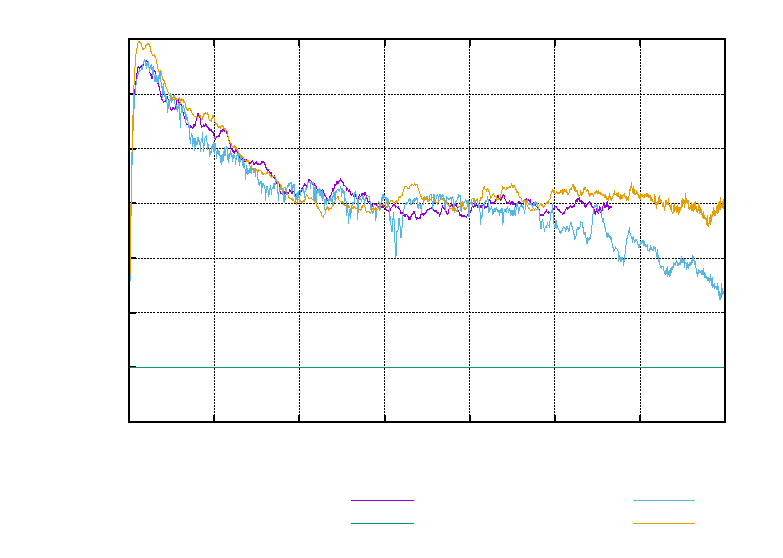
\includegraphics[width={360.00bp},height={252.00bp}]{./vraiInertie}}%
    \gplfronttext
  \end{picture}%
\endgroup
}
        \caption{Recalcul $I$ exact ($\sigma_3 = 300\,\text{kPa}$, $R = 0.005\,\text{m}$)}
    \end{figure}
    \begin{columns}
        \begin{column}{0.45\textwidth}
            \begin{table}[h]
                \centering
                \begin{tabular}{c c}
                    \hline
                    $v$ & $I$                  \\
                    \hline
                    0.1 & $4.4 \times 10^{-4}$ \\
                    10  & $4.4 \times 10^{-2}$ \\
                    \hline
                \end{tabular}
                \caption{Calcul précédent approximatif}
            \end{table}
        \end{column}
        \begin{column}{0.45\textwidth}
            \begin{table}[h]
                \centering
                \begin{tabular}{c c}
                    \hline
                    $v$    & $I$       \\
                    \hline
                    0.0227 & $10^{-4}$ \\
                    2.27   & $10^{-2}$ \\
                    \hline
                \end{tabular}
                \caption{Calcul exact}
            \end{table}
        \end{column}
    \end{columns}
\end{frame}

\begin{frame}{Les résultats varient de manière très sensible avec $I$}
    \begin{columns}
        \begin{column}{0.5\textwidth}
            \begin{figure}[h]
                \centering
                \scalebox{0.5}{% GNUPLOT: LaTeX picture with Postscript
\begingroup
  \makeatletter
  \providecommand\color[2][]{%
    \GenericError{(gnuplot) \space\space\space\@spaces}{%
      Package color not loaded in conjunction with
      terminal option `colourtext'%
    }{See the gnuplot documentation for explanation.%
    }{Either use 'blacktext' in gnuplot or load the package
      color.sty in LaTeX.}%
    \renewcommand\color[2][]{}%
  }%
  \providecommand\includegraphics[2][]{%
    \GenericError{(gnuplot) \space\space\space\@spaces}{%
      Package graphicx or graphics not loaded%
    }{See the gnuplot documentation for explanation.%
    }{The gnuplot epslatex terminal needs graphicx.sty or graphics.sty.}%
    \renewcommand\includegraphics[2][]{}%
  }%
  \providecommand\rotatebox[2]{#2}%
  \@ifundefined{ifGPcolor}{%
    \newif\ifGPcolor
    \GPcolortrue
  }{}%
  \@ifundefined{ifGPblacktext}{%
    \newif\ifGPblacktext
    \GPblacktextfalse
  }{}%
  % define a \g@addto@macro without @ in the name:
  \let\gplgaddtomacro\g@addto@macro
  % define empty templates for all commands taking text:
  \gdef\gplbacktext{}%
  \gdef\gplfronttext{}%
  \makeatother
  \ifGPblacktext
    % no textcolor at all
    \def\colorrgb#1{}%
    \def\colorgray#1{}%
  \else
    % gray or color?
    \ifGPcolor
      \def\colorrgb#1{\color[rgb]{#1}}%
      \def\colorgray#1{\color[gray]{#1}}%
      \expandafter\def\csname LTw\endcsname{\color{white}}%
      \expandafter\def\csname LTb\endcsname{\color{black}}%
      \expandafter\def\csname LTa\endcsname{\color{black}}%
      \expandafter\def\csname LT0\endcsname{\color[rgb]{1,0,0}}%
      \expandafter\def\csname LT1\endcsname{\color[rgb]{0,1,0}}%
      \expandafter\def\csname LT2\endcsname{\color[rgb]{0,0,1}}%
      \expandafter\def\csname LT3\endcsname{\color[rgb]{1,0,1}}%
      \expandafter\def\csname LT4\endcsname{\color[rgb]{0,1,1}}%
      \expandafter\def\csname LT5\endcsname{\color[rgb]{1,1,0}}%
      \expandafter\def\csname LT6\endcsname{\color[rgb]{0,0,0}}%
      \expandafter\def\csname LT7\endcsname{\color[rgb]{1,0.3,0}}%
      \expandafter\def\csname LT8\endcsname{\color[rgb]{0.5,0.5,0.5}}%
    \else
      % gray
      \def\colorrgb#1{\color{black}}%
      \def\colorgray#1{\color[gray]{#1}}%
      \expandafter\def\csname LTw\endcsname{\color{white}}%
      \expandafter\def\csname LTb\endcsname{\color{black}}%
      \expandafter\def\csname LTa\endcsname{\color{black}}%
      \expandafter\def\csname LT0\endcsname{\color{black}}%
      \expandafter\def\csname LT1\endcsname{\color{black}}%
      \expandafter\def\csname LT2\endcsname{\color{black}}%
      \expandafter\def\csname LT3\endcsname{\color{black}}%
      \expandafter\def\csname LT4\endcsname{\color{black}}%
      \expandafter\def\csname LT5\endcsname{\color{black}}%
      \expandafter\def\csname LT6\endcsname{\color{black}}%
      \expandafter\def\csname LT7\endcsname{\color{black}}%
      \expandafter\def\csname LT8\endcsname{\color{black}}%
    \fi
  \fi
    \setlength{\unitlength}{0.0500bp}%
    \ifx\gptboxheight\undefined%
      \newlength{\gptboxheight}%
      \newlength{\gptboxwidth}%
      \newsavebox{\gptboxtext}%
    \fi%
    \setlength{\fboxrule}{0.5pt}%
    \setlength{\fboxsep}{1pt}%
    \definecolor{tbcol}{rgb}{1,1,1}%
\begin{picture}(7200.00,5040.00)%
    \gplgaddtomacro\gplbacktext{%
      \csname LTb\endcsname%%
      \put(946,1144){\makebox(0,0)[r]{\strut{}$0$}}%
      \csname LTb\endcsname%%
      \put(946,2063){\makebox(0,0)[r]{\strut{}$500$}}%
      \csname LTb\endcsname%%
      \put(946,2982){\makebox(0,0)[r]{\strut{}$1000$}}%
      \csname LTb\endcsname%%
      \put(946,3900){\makebox(0,0)[r]{\strut{}$1500$}}%
      \csname LTb\endcsname%%
      \put(946,4819){\makebox(0,0)[r]{\strut{}$2000$}}%
      \csname LTb\endcsname%%
      \put(1078,924){\makebox(0,0){\strut{}$0$}}%
      \csname LTb\endcsname%%
      \put(1896,924){\makebox(0,0){\strut{}$10$}}%
      \csname LTb\endcsname%%
      \put(2714,924){\makebox(0,0){\strut{}$20$}}%
      \csname LTb\endcsname%%
      \put(3532,924){\makebox(0,0){\strut{}$30$}}%
      \csname LTb\endcsname%%
      \put(4349,924){\makebox(0,0){\strut{}$40$}}%
      \csname LTb\endcsname%%
      \put(5167,924){\makebox(0,0){\strut{}$50$}}%
      \csname LTb\endcsname%%
      \put(5985,924){\makebox(0,0){\strut{}$60$}}%
      \csname LTb\endcsname%%
      \put(6803,924){\makebox(0,0){\strut{}$70$}}%
    }%
    \gplgaddtomacro\gplfronttext{%
      \csname LTb\endcsname%%
      \put(341,2981){\rotatebox{-270}{\makebox(0,0){\strut{}q (kPa)}}}%
      \put(3940,594){\makebox(0,0){\strut{}$\varepsilon_{yy}$ (\%)}}%
      \csname LTb\endcsname%%
      \put(3085,393){\makebox(0,0)[r]{\strut{}$I = 10^{-4}$}}%
      \csname LTb\endcsname%%
      \put(3085,173){\makebox(0,0)[r]{\strut{}$I = 10^{-3}$}}%
      \csname LTb\endcsname%%
      \put(4996,393){\makebox(0,0)[r]{\strut{}$I = 10^{-2}$}}%
      \csname LTb\endcsname%%
      \put(4996,173){\makebox(0,0)[r]{\strut{}$I = 10^{-1}$}}%
    }%
    \gplbacktext
    \put(0,0){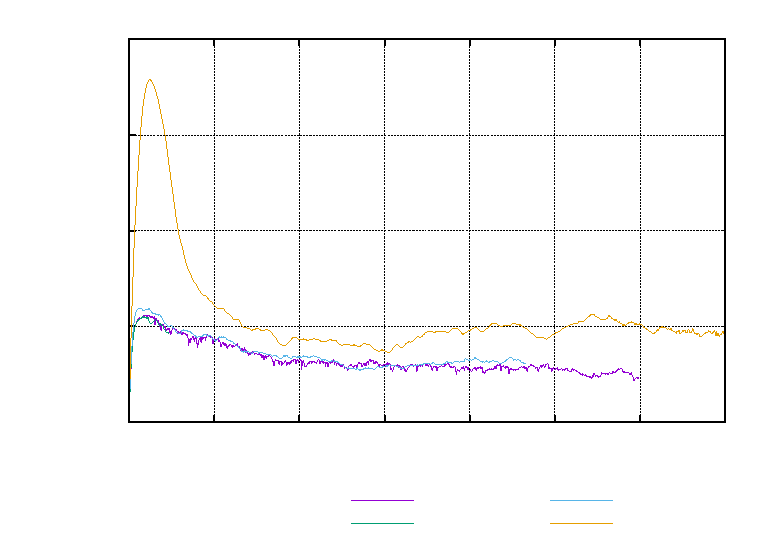
\includegraphics[width={360.00bp},height={252.00bp}]{./veriteI0terms}}%
    \gplfronttext
  \end{picture}%
\endgroup
}
                \caption{Contrainte - Déformation DEM (changer la vitesse)}
            \end{figure}
        \end{column}
        \begin{column}{0.5\textwidth}
            \begin{figure}[h]
                \centering
                \scalebox{0.5}{% GNUPLOT: LaTeX picture with Postscript
\begingroup
  \makeatletter
  \providecommand\color[2][]{%
    \GenericError{(gnuplot) \space\space\space\@spaces}{%
      Package color not loaded in conjunction with
      terminal option `colourtext'%
    }{See the gnuplot documentation for explanation.%
    }{Either use 'blacktext' in gnuplot or load the package
      color.sty in LaTeX.}%
    \renewcommand\color[2][]{}%
  }%
  \providecommand\includegraphics[2][]{%
    \GenericError{(gnuplot) \space\space\space\@spaces}{%
      Package graphicx or graphics not loaded%
    }{See the gnuplot documentation for explanation.%
    }{The gnuplot epslatex terminal needs graphicx.sty or graphics.sty.}%
    \renewcommand\includegraphics[2][]{}%
  }%
  \providecommand\rotatebox[2]{#2}%
  \@ifundefined{ifGPcolor}{%
    \newif\ifGPcolor
    \GPcolortrue
  }{}%
  \@ifundefined{ifGPblacktext}{%
    \newif\ifGPblacktext
    \GPblacktextfalse
  }{}%
  % define a \g@addto@macro without @ in the name:
  \let\gplgaddtomacro\g@addto@macro
  % define empty templates for all commands taking text:
  \gdef\gplbacktext{}%
  \gdef\gplfronttext{}%
  \makeatother
  \ifGPblacktext
    % no textcolor at all
    \def\colorrgb#1{}%
    \def\colorgray#1{}%
  \else
    % gray or color?
    \ifGPcolor
      \def\colorrgb#1{\color[rgb]{#1}}%
      \def\colorgray#1{\color[gray]{#1}}%
      \expandafter\def\csname LTw\endcsname{\color{white}}%
      \expandafter\def\csname LTb\endcsname{\color{black}}%
      \expandafter\def\csname LTa\endcsname{\color{black}}%
      \expandafter\def\csname LT0\endcsname{\color[rgb]{1,0,0}}%
      \expandafter\def\csname LT1\endcsname{\color[rgb]{0,1,0}}%
      \expandafter\def\csname LT2\endcsname{\color[rgb]{0,0,1}}%
      \expandafter\def\csname LT3\endcsname{\color[rgb]{1,0,1}}%
      \expandafter\def\csname LT4\endcsname{\color[rgb]{0,1,1}}%
      \expandafter\def\csname LT5\endcsname{\color[rgb]{1,1,0}}%
      \expandafter\def\csname LT6\endcsname{\color[rgb]{0,0,0}}%
      \expandafter\def\csname LT7\endcsname{\color[rgb]{1,0.3,0}}%
      \expandafter\def\csname LT8\endcsname{\color[rgb]{0.5,0.5,0.5}}%
    \else
      % gray
      \def\colorrgb#1{\color{black}}%
      \def\colorgray#1{\color[gray]{#1}}%
      \expandafter\def\csname LTw\endcsname{\color{white}}%
      \expandafter\def\csname LTb\endcsname{\color{black}}%
      \expandafter\def\csname LTa\endcsname{\color{black}}%
      \expandafter\def\csname LT0\endcsname{\color{black}}%
      \expandafter\def\csname LT1\endcsname{\color{black}}%
      \expandafter\def\csname LT2\endcsname{\color{black}}%
      \expandafter\def\csname LT3\endcsname{\color{black}}%
      \expandafter\def\csname LT4\endcsname{\color{black}}%
      \expandafter\def\csname LT5\endcsname{\color{black}}%
      \expandafter\def\csname LT6\endcsname{\color{black}}%
      \expandafter\def\csname LT7\endcsname{\color{black}}%
      \expandafter\def\csname LT8\endcsname{\color{black}}%
    \fi
  \fi
    \setlength{\unitlength}{0.0500bp}%
    \ifx\gptboxheight\undefined%
      \newlength{\gptboxheight}%
      \newlength{\gptboxwidth}%
      \newsavebox{\gptboxtext}%
    \fi%
    \setlength{\fboxrule}{0.5pt}%
    \setlength{\fboxsep}{1pt}%
    \definecolor{tbcol}{rgb}{1,1,1}%
\begin{picture}(7200.00,5040.00)%
    \gplgaddtomacro\gplbacktext{%
      \csname LTb\endcsname%%
      \put(946,1144){\makebox(0,0)[r]{\strut{}$0$}}%
      \csname LTb\endcsname%%
      \put(946,2063){\makebox(0,0)[r]{\strut{}$500$}}%
      \csname LTb\endcsname%%
      \put(946,2982){\makebox(0,0)[r]{\strut{}$1000$}}%
      \csname LTb\endcsname%%
      \put(946,3900){\makebox(0,0)[r]{\strut{}$1500$}}%
      \csname LTb\endcsname%%
      \put(946,4819){\makebox(0,0)[r]{\strut{}$2000$}}%
      \csname LTb\endcsname%%
      \put(1078,924){\makebox(0,0){\strut{}$0$}}%
      \csname LTb\endcsname%%
      \put(1896,924){\makebox(0,0){\strut{}$10$}}%
      \csname LTb\endcsname%%
      \put(2714,924){\makebox(0,0){\strut{}$20$}}%
      \csname LTb\endcsname%%
      \put(3532,924){\makebox(0,0){\strut{}$30$}}%
      \csname LTb\endcsname%%
      \put(4349,924){\makebox(0,0){\strut{}$40$}}%
      \csname LTb\endcsname%%
      \put(5167,924){\makebox(0,0){\strut{}$50$}}%
      \csname LTb\endcsname%%
      \put(5985,924){\makebox(0,0){\strut{}$60$}}%
      \csname LTb\endcsname%%
      \put(6803,924){\makebox(0,0){\strut{}$70$}}%
    }%
    \gplgaddtomacro\gplfronttext{%
      \csname LTb\endcsname%%
      \put(341,2981){\rotatebox{-270}{\makebox(0,0){\strut{}q (kPa)}}}%
      \put(3940,594){\makebox(0,0){\strut{}$\varepsilon_{yy}$ (\%)}}%
      \csname LTb\endcsname%%
      \put(3085,393){\makebox(0,0)[r]{\strut{}$I = 10^{-4}$}}%
      \csname LTb\endcsname%%
      \put(3085,173){\makebox(0,0)[r]{\strut{}$I = 10^{-3}$}}%
      \csname LTb\endcsname%%
      \put(4996,393){\makebox(0,0)[r]{\strut{}$I = 10^{-2}$}}%
      \csname LTb\endcsname%%
      \put(4996,173){\makebox(0,0)[r]{\strut{}$I = 10^{-1}$}}%
    }%
    \gplbacktext
    \put(0,0){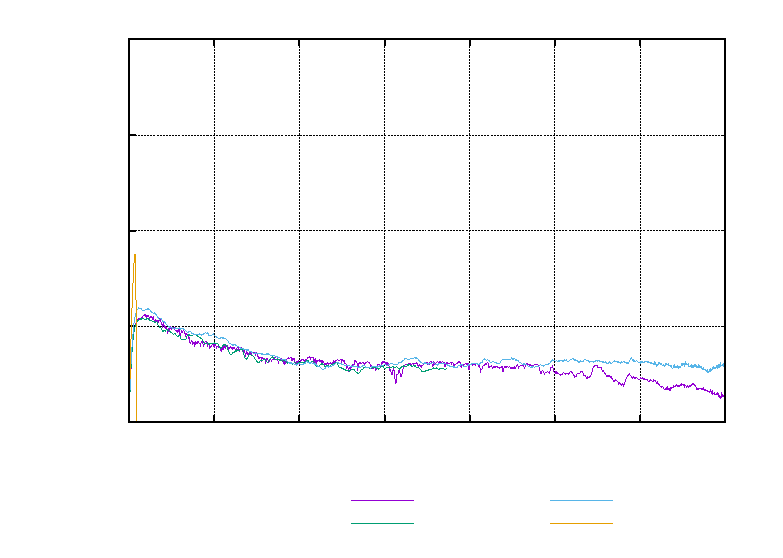
\includegraphics[width={360.00bp},height={252.00bp}]{./VeriteI2terms}}%
    \gplfronttext
  \end{picture}%
\endgroup
}
                \caption{Bruyant concernant pas de temps MPM (avant)}
            \end{figure}
        \end{column}
    \end{columns}
    $I = 10^{-2}$ se marche maintenant
\end{frame}

\begin{frame}{Souci concernant demi-vélocité}
    \begin{itemize}
        \item Si $\Delta t$ est très petit et $a(t) \approx a(t+\Delta t)$, on “perd” peut-être la moitié de l'incrément de $v(t+\Delta t)$.
        \item Pour des essais triaxiaux à chargement rapide, cette différence pourrait devenir critique.
        \item Lors du calcul des contraintes avec le terme dynamique $(mv^2)$, l'erreur peut s'amplifier, possiblement proportionnellement au carré de la vitesse.
    \end{itemize}

    \textbf{Formules de référence du Verlet Velocité :}
    \[
        \text{Demi-pas vitesse: } v(t + 0.5\Delta t) = v(t) + 0.5\,\Delta t\, a(t)
    \]
    \[
        \text{Vitesse au pas entier: } v(t + \Delta t) = v(t) + 0.5\,\Delta t \,[a(t) + a(t+\Delta t)]
    \]

    \begin{figure}[h]
        \centering
        \scalebox{0.15}{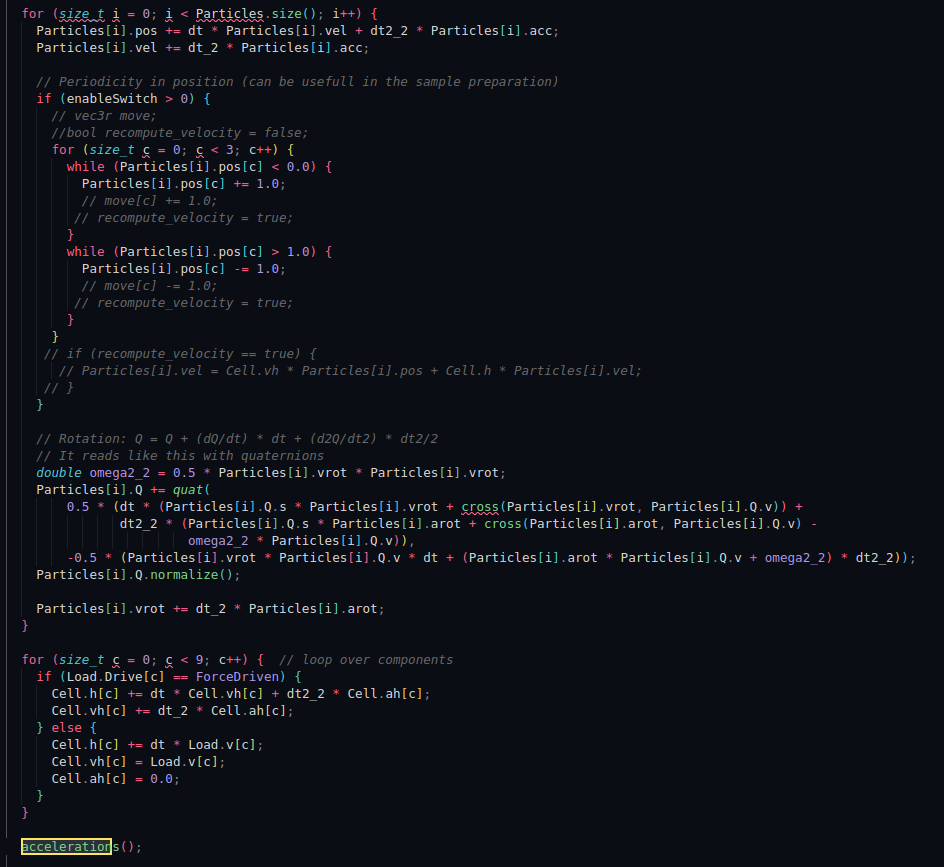
\includegraphics{demiVelocite.png}}
        \caption{La programme}
    \end{figure}
\end{frame}

\begin{frame}{Hors de sujet}
    \begin{figure}[h]
        \centering
        \scalebox{0.15}{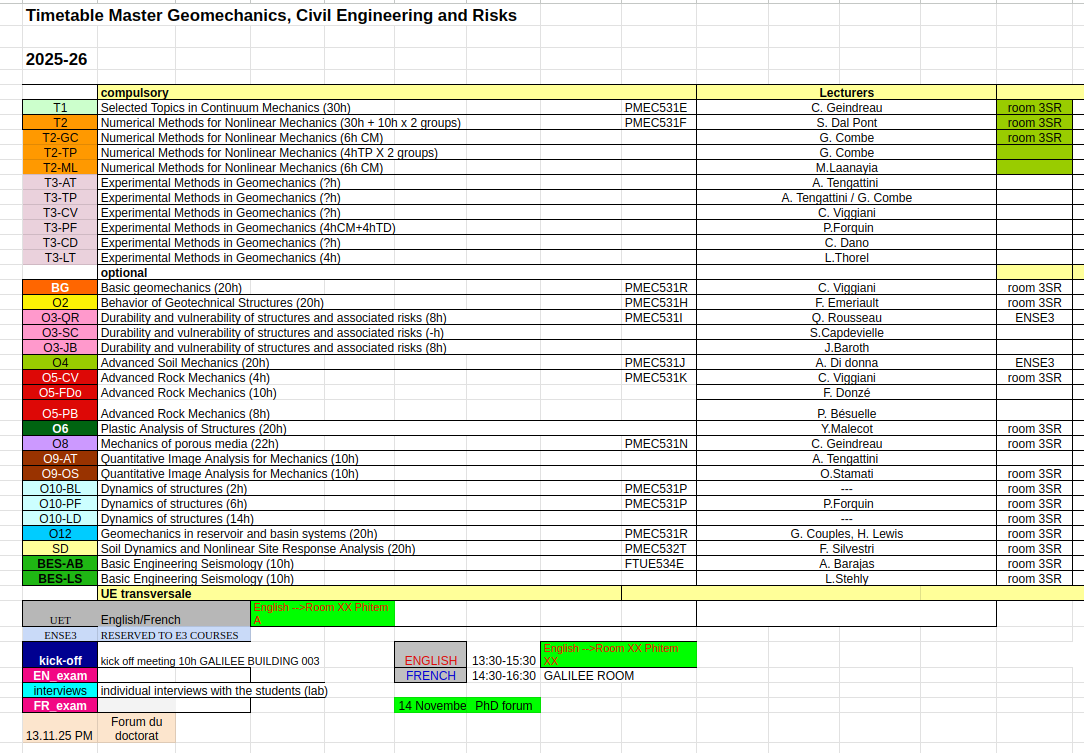
\includegraphics{Courses.png}}
        \caption{Cours de master}
    \end{figure}
    \begin{figure}[h]
        \centering
        \scalebox{0.095}{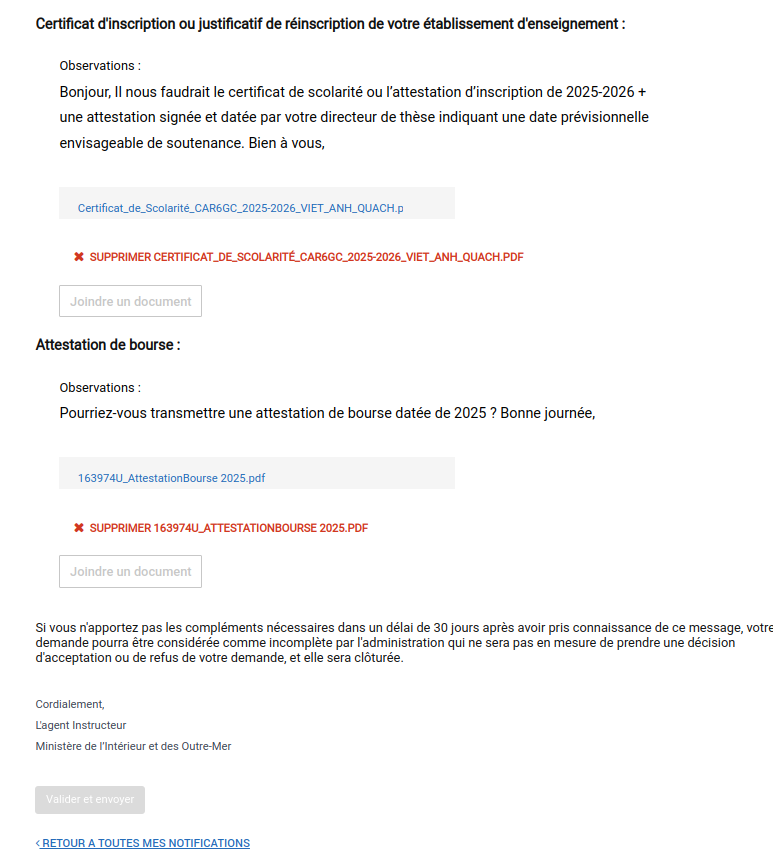
\includegraphics{DatePrvision.png}}
        \caption{Fonction de comparison}
    \end{figure}
\end{frame}

\end{document}
